\chapter{Svolgimento dello \textit{stage}}
    \section{Conoscenza del dominio di applicazione}
    Le attività iniziali del progetto hanno previsto un'immersione approfondita nel dominio applicativo, costituito da un ecosistema manifatturiero dedicato alla produzione di beni per aziende terze. Il sistema in esame si configura come una soluzione trasversale e implementabile in molteplici realtà produttive che adottano metodologie operative simili. L'architettura attuale è basata sulla piattaforma SAI, mentre l'obiettivo dello \textit{stage} è stato quello di condurre un'analisi completa finalizzata alla rimodellazione del dominio.

    \vspace{0.2 em}
    \noindent Le caratteristiche principali del sistema attuale sono:

    \begin{itemize}
        \item \textbf{tracciabilità delle risorse umane}: il sistema mantiene un registro completo del personale operativo, con identificazione univoca di ciascun lavoratore all'interno dell'ecosistema informativo;

        \item \textbf{monitoraggio del processo produttivo}: ogni fase della catena di lavorazione è dettagliatamente documentata, con registrazione sistematica dello stato avanzamento lavori per ciascuna operazione in corso;

        \item \textbf{gestione dell'inventario}: implementazione di meccanismi di controllo delle materie prime, con funzionalità di rilevamento delle soglie critiche e conseguente attivazione di processi di approvvigionamento, alcuni dei quali completamente automatizzati;

        \item \textbf{amministrazione integrata}: il sistema incorpora moduli per la gestione contabile, l'elaborazione documentale e la pianificazione logistica del trasporto.

    \end{itemize}
    
    \vspace{0.2 em}
    \noindent Il progetto di \textit{stage} si è focalizzato principalmente sull'analisi approfondita del dominio applicativo, con l'obiettivo di aggiornare e ridefinire il modello esistente. Questo processo ha previsto l'identificazione e la delimitazione dei \textit{bounded contexts} secondo i principi del \textit{Domain-Driven Design}, cercando di mantenere una rappresentazione chiara e coerente delle diverse aree funzionali del sistema. Le attività successive hanno riguardato la formalizzazione dei requisiti funzionali e non funzionali, definendo così i confini tecnici e prestazionali necessari per lo sviluppo del microservizio. Come anticipato nella Sezione 1.6.2, le situazioni descritte possono costituire un modello di dominio completo.  

    \vspace{0.2 em}
    \noindent L'obiettivo principale del progetto di \textit{stage} era individuare un modello di dominio specifico e svilupparne un prototipo. Dopo un'attenta valutazione, è stato scelto il \textbf{monitoraggio del processo produttivo} come ambito di intervento. Durante il lavoro, ho potuto constatare quanto sia complesso separare completamente i modelli di dominio, poiché alcuni si intersecano inevitabilmente. Questo mi ha portato alla consapevolezza che non esiste una soluzione perfetta in senso assoluto, bensì un compromesso tra le diverse esigenze e realtà operative. 
    
    
    \section{Attività svolte}
        \subsection{Analisi dei requisiti}
        Tra i vari modelli di dominio individuati, è stato dunque selezionato quello relativo al \textbf{monitoraggio del processo produttivo}.

        \vspace{0.2 em}
        \noindent L'analisi dei requisiti è stata condotta in collaborazione con il \textit{Product Owner}. L'obiettivo primario è stato comprendere approfonditamente le esigenze e le aspettative degli utenti finali, con particolare attenzione al contesto preesistente nel sistema monolitico.
        
        \vspace{0.2 em}
        \noindent Per raggiungere una definizione precisa dei requisiti, si è adottata la metodologia delle \textit{User Story}, uno strumento concettuale che consente di descrivere sinteticamente e in forma narrativa i bisogni specifici degli utenti. Attraverso la redazione di un documento articolato che raccoglieva tali \textit{User Story}, mi è stato possibile procedere all'identificazione dei requisiti funzionali iniziali. Queste sono state sviluppate in modo incrementale, parallelamente all'approfondimento della mia conoscenza del dominio specifico.
        
        \vspace{0.2 em}
        \noindent Un elemento metodologico di particolare rilevanza è stato l'utilizzo di prototipi dimostrativi. Tali strumenti si sono rivelati estremamente efficaci nel facilitare la visualizzazione della soluzione tanto per il cliente quanto per il \textit{team} di sviluppo, contribuendo a dissipare eventuali ambiguità concettuali.

        \vspace{0.2 em}
        \noindent Nello specifico le attività di analisi hanno previsto un'accurata ispezione da remoto dei sistemi informativi presso l'impianto industriale destinatario del servizio. Tale indagine mi ha consentito di acquisire una comprensione approfondita della giornata lavorativa tipo, fornendo elementi informativi che hanno supportato lo sviluppo nella formulazione di nuove \textit{User Story} e nell'individuazione di questioni critiche da approfondire mediante confronto con i rappresentanti e i consulenti. Io ho interagito solo con il \textit{Product Owne}r, infatti è solo quest'ultimo che ha contatto diretto con l'azienda cliente.

        \vspace{0.2 em}
        \noindent Partendo dall'esame approfondito della situazione rappresentata nella Figura \ref{fig:Dominio}. Tale attività ha permesso di delineare con precisione le necessità operative e gli obiettivi funzionali, costituendo la base per lo sviluppo del prototipo.

        \begin{figure}
            \centering
            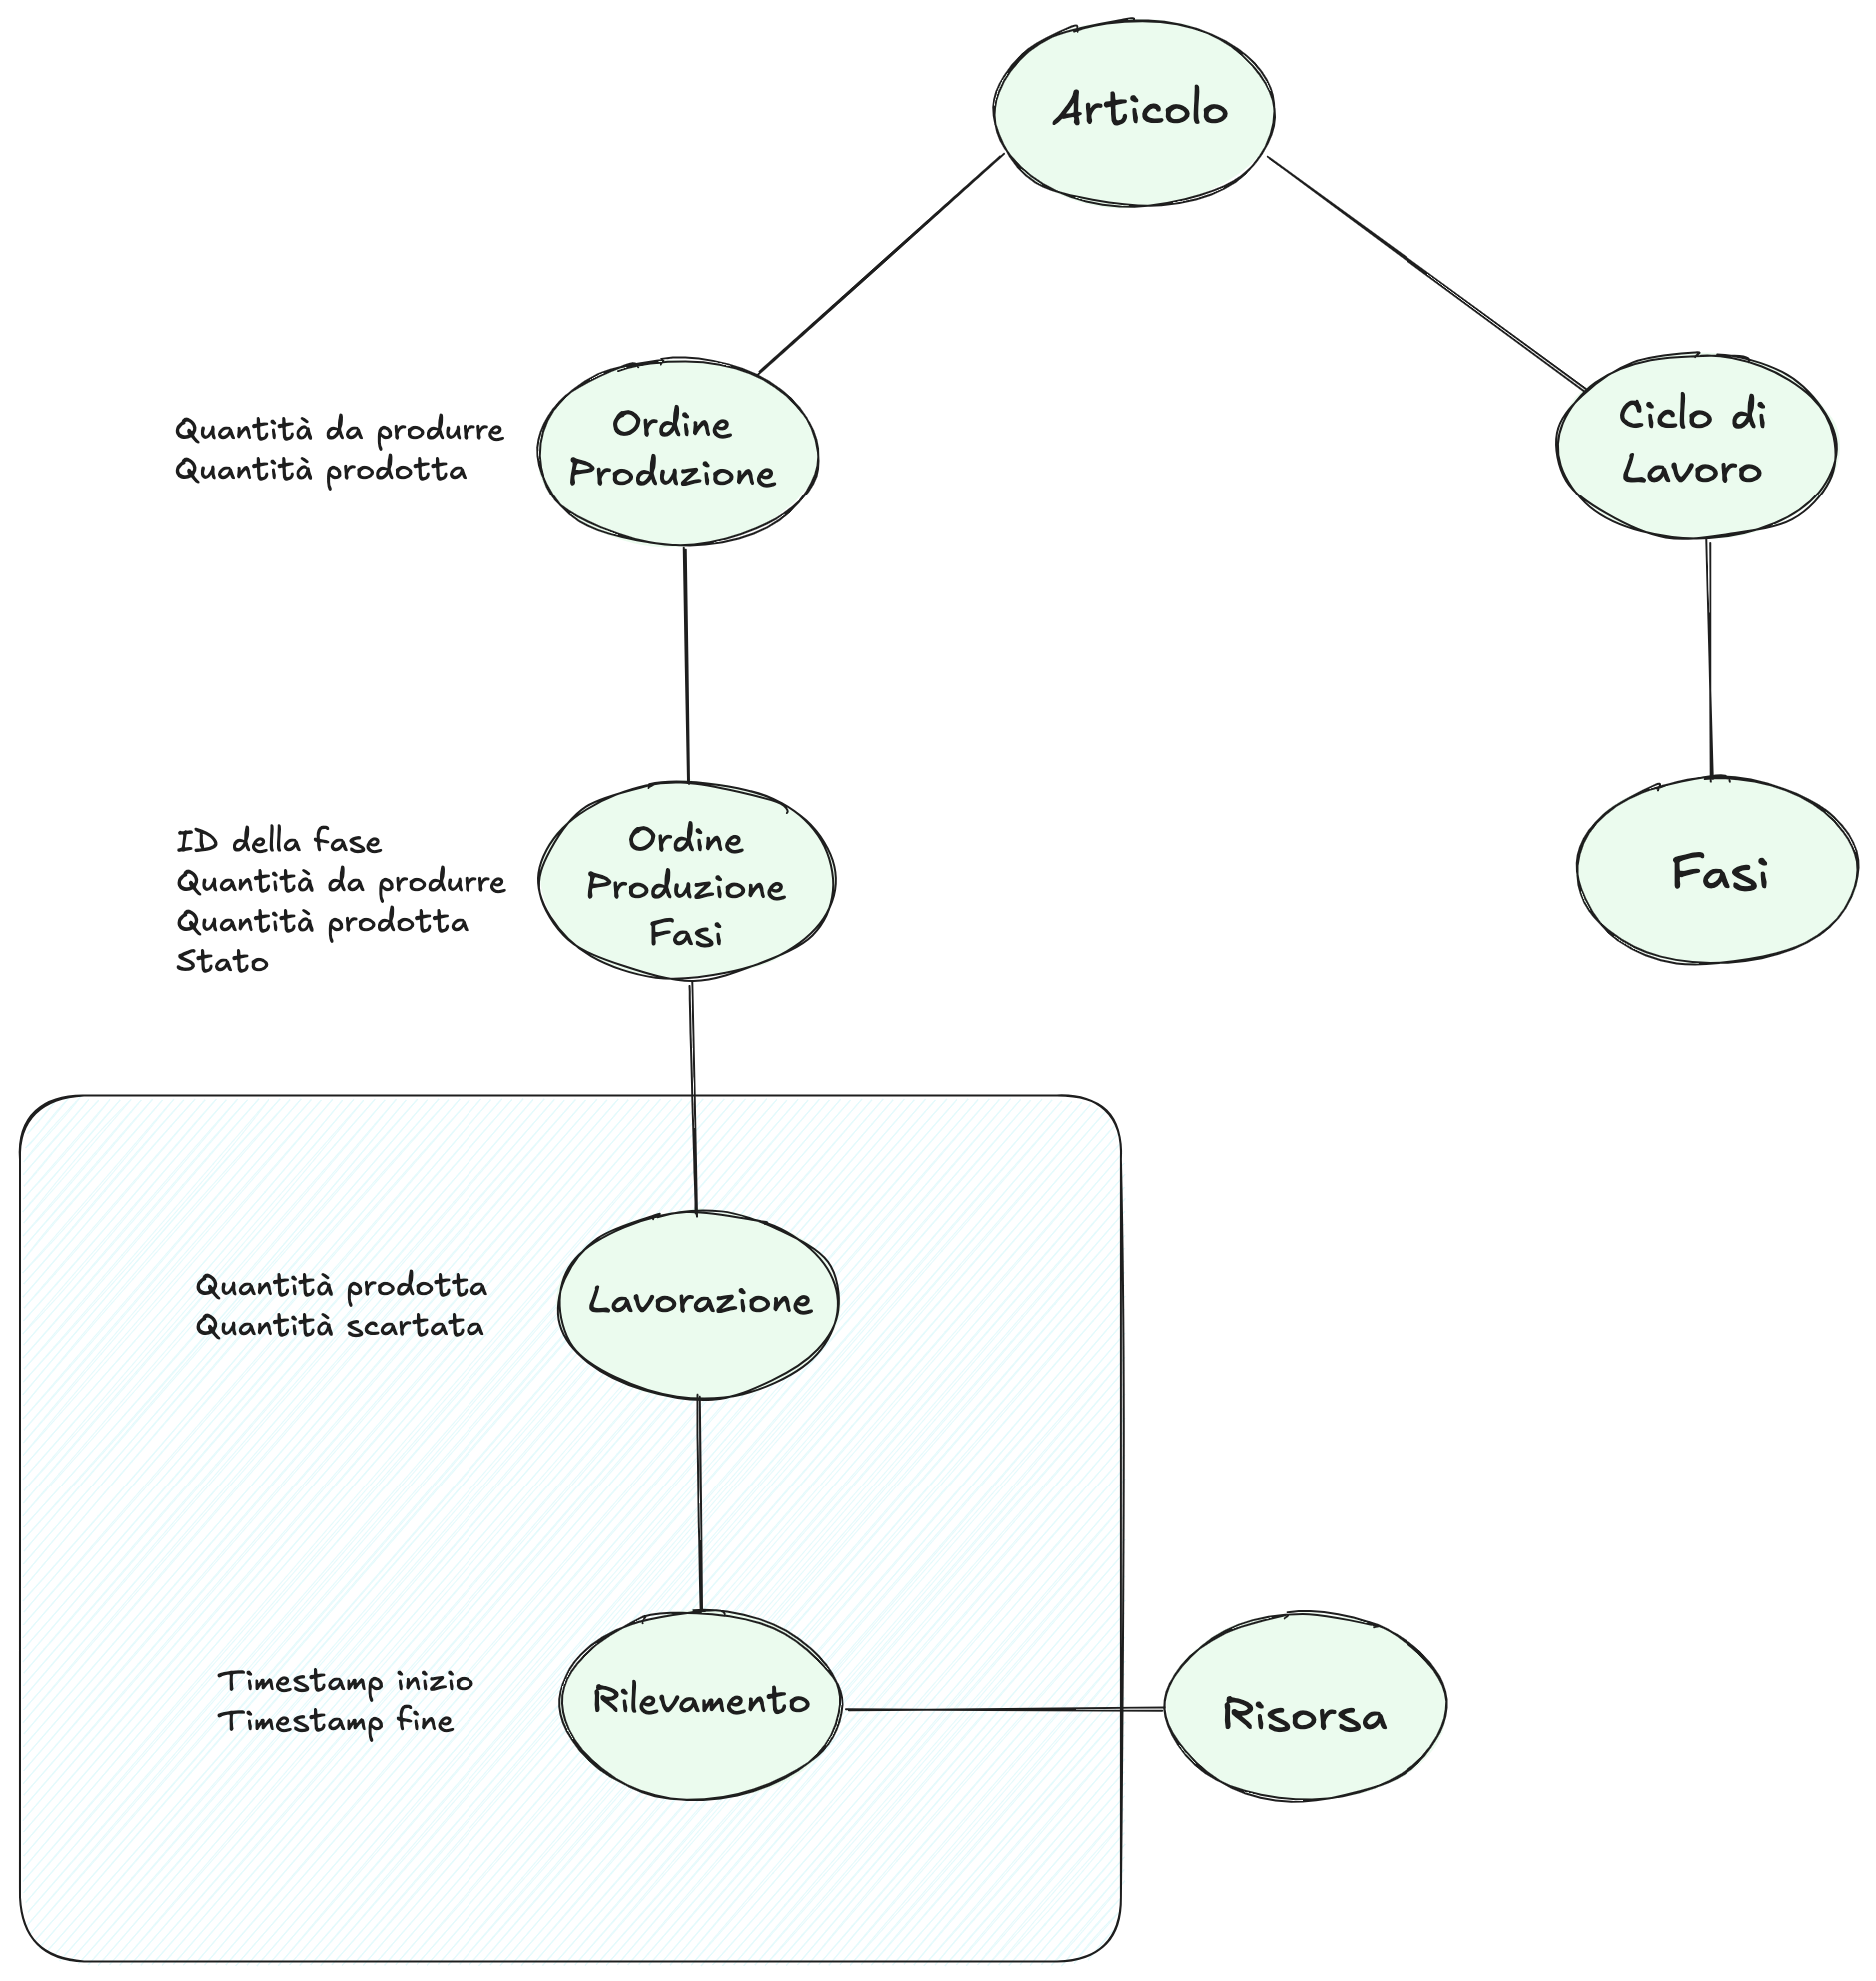
\includegraphics[width=0.6\linewidth]{BCS-Tessi//images/Dominio.png}
            \caption[Modello di dominio preso in esame]{Schema visuale del modello di dominio preso in esame durante l'attività di analisi dei requisiti}
            \label{fig:Dominio}
        \end{figure}

        \vspace{0.2 em}
        \noindent L'immagine descrive una situazione reale semplificata con cui l'azienda si interfaccia: la gestione della produzione di un certo \texttt{Articolo} finito, la cui produzione prevede un certo \texttt{CicloDiLavoro} composto da diverse \texttt{Fasi} che sono predefinite. Consideriamo ogni componente corrispondere a un \textit{bounded context}.
        Nello specifico: 
        \begin{itemize}
            \item La produzione di un \texttt{Articolo} richiede un \texttt{OrdineProduzione}, che rappresenta la quantità da produrre e la quantità prodotta.
            \item \texttt{OrdineProduzioneFasi} tiene traccia dello stato di avanzamento della produzione, monitorando quante unità sono state prodotte in relazione a ciascuna \texttt{Fase} e in base alla disponibilità di materiali. Questo strumento è fondamentale per garantire che la produzione si svolga correttamente, considerando anche eventuali imprevisti come la scarsità di risorse. Infatti, se la quantità richiesta non può essere raggiunta a causa di una carenza di materiali, il conteggio si ferma automaticamente quando il numero di unità programmato è stato raggiunto oppure manualmente quando le risorse sono state esaurite. Questo processo tiene conto di diversi fattori, come la quantità da produrre, quella effettivamente prodotta e lo stato del processo (aperto, in corso, chiuso), fornendo un controllo dettagliato del progresso produttivo;
            \item Il riquadro nell'immagine include i \textit{bounded context} presi in analisi, in particolare il processo di \texttt{Rilevamento}, che prevede l'inserimento dei dati da parte dei lavoratori. Ogni lavoratore deve segnare, attraverso un \textit{badge}, l'inizio e la fine del proprio turno di lavoro, insieme al numero di pezzi prodotti in base alla fase di \texttt{Lavorazione} in corso. Una volta completata una fase di \texttt{Rilevamento}, questa azione porta all'avanzamento della \texttt{Lavorazione}, la quale tiene traccia sia della quantità prodotta che della quantità scartata, monitorando quindi la qualità del processo;
            \item Una \texttt{Risorsa} è rappresentata da tutti gli elementi necessari per il completamento di una \texttt{Fase} produttiva: include l'operaio che esegue il lavoro, la macchina utilizzata per ciascuna fase di produzione, la fase stessa, il numero di unità prodotte, nonché l'ora di inizio e di fine di ciascun intervento.
        \end{itemize}

        \vspace{0.2 em}
        \noindent Il problema principale è far comunicare in tempo reale \texttt{Rilevamento} e \texttt{OrdineProduzioneFasi}, senza che quest'ultimo debba essere portato all'interno del microservizio che individuiamo come \texttt{MS\_Rilevamento}.

        \vspace{0.2 em}
        \noindent La soluzione ideale infatti sarebbe quella di includere \texttt{OrdineProduzione} e \texttt{OrdineProduzioneFasi} nell'unico microservizio \texttt{MS\_Rilevamento}. Questo perché secondo i principi del \textit{Domain-Driven Design} la divisione in \textit{bounded contexts} dovrebbe attuare una scomposizione in microservizi che siano poco accoppiati tra di loro. In questo caso invece c'è un alto grado di accoppiamento tra i \textit{bounded context} appena citati e  \texttt{Lavorazione}, quindi scomporli in servizi differenti non è in linea con i principi DDD\footnote{E. Evans, Domain-Driven Design: Tackling Complexity in the Heart of Software, Addison-Wesley, 2003}.

        \vspace{0.2 em}
        \noindent Questa soluzione non è applicabile al momento perché il monolite è strettamente collegato in vari punti con \texttt{OrdineProduzione} e con \texttt{OrdineProduzioneFasi}. La priorità è dunque estrarre \texttt{Rilevamento} e \texttt{Lavorazione} in un unico servizio, e in un secondo momento completare la divisione ideale.

        \vspace{0.2 em}
        \noindent Un altro problema è rappresentato dalla necessità di \texttt{MS\_Rilevamento} di leggere dei dati da due fonti. Per monitorare lo stato di una \texttt{Lavorazione} in relazione a \texttt{OrdineProduzione}, è necessario confrontare i dati provenienti sia dal microservizio, sia dal monolite. Questo perché altrimenti non è possibile accedere ai dati essenziali dell'ordine della fase da lavorare, senza portare \texttt{OrdineProduzione} all'interno di \texttt{MS\_Rilevamento}. Come farlo sarà oggetto della sezione successiva. 

        \vspace{0.2 em}
        \noindent Nell'ambito del mio \textit{stage} didattico, la complessità del dominio applicativo e i vincoli temporali intrinseci al progetto hanno determinato la necessità di selezionare i requisiti individuati in base alle priorità.

        \vspace{0.2 em}
        \noindent Sebbene l'implementazione si sia concentrata su un sottoinsieme specifico delle entità individuate, ho compreso comunque tutti i requisiti che ho individuato nelle attività di analisi. Questa scelta metodologica ha consentito di mantenere una visione olistica del progetto, garantendo al contempo una realizzazione maggiormente sostenibile e allineata con le risorse disponibili.

        \vspace{0.2 em}
        \noindent I requisiti individuati li ho definiti seguendo le linee guida aziendali, assicurando così una perfetta coerenza con gli \textit{standard} e le aspettative di SogeaSoft S.r.l. La Tabella \ref{tab:requisiti} rappresenta una sintesi concisa di tali requisiti, offrendo una panoramica strutturata degli obiettivi progettuali complessivi. 

        \begin{table}[H]
        \centering
        \renewcommand{\arraystretch}{1.8} % Increase row height by 50%
        \begin{tabular}{|l|c|c|c|}
        \hline
        \rowcolor[gray]{0.95}
        \textbf{Tipo} & \textbf{Obbligatori} & \textbf{Desiderabili} & \textbf{Opzionali} \\
        \hline
        Dominio & 23 & 0 & 0 \\
        \hline
        Funzioni & 89 & 12 & 8 \\
        \hline
        Prestazioni & 0 & 0 & 7 \\
        \hline
        Sincronizzazione & 5 & 2 & 1 \\
        \hline
        Progettazione & 12 & 0 & 0 \\
        \hline
        \multicolumn{4}{|c|}{159 requisiti totali}\\
        \hline
        \end{tabular}
        \caption[Tabella dei requisiti individuati]{Tabella dei requisiti individuati durante l'attività di analisi dei requisiti}
        \label{tab:requisiti}
        \end{table}

        \subsection{Progettazione}
        Durante il mio \textit{stage}, l'analisi dei requisiti e le attività di progettazione si sono sviluppate in modo parallelo. Con l'aumentare della mia conoscenza del dominio applicativo e l'individuazione dei requisiti, la progettazione, guidata dal \textit{Product Owner}, è avvenuta in modo naturale, senza una netta separazione tra le due attività.  

        \vspace{0.2 em}
        \noindent Poiché la progettazione consiste nel definire come realizzare concretamente quanto emerso dall'analisi dei requisiti, questo capitolo si concentrerà sulla descrizione dei \textit{pattern} identificati e delle soluzioni architetturali adottate per soddisfare i requisiti individuati.

        \vspace{0.2 em}
        \noindent La soluzione individuata è rappresentata nella Figura \ref{fig:progettazione} e rappresenta il modo in cui \texttt{MS\_} \texttt{Rilevamento} potrà comunicare con SAI attraverso un \texttt{MS\_Middleware}. Questo rappresenta molto bene il piano di migrazione visibile nella Figura \ref{fig:migrazione}.
        
        \begin{figure}
            \centering
            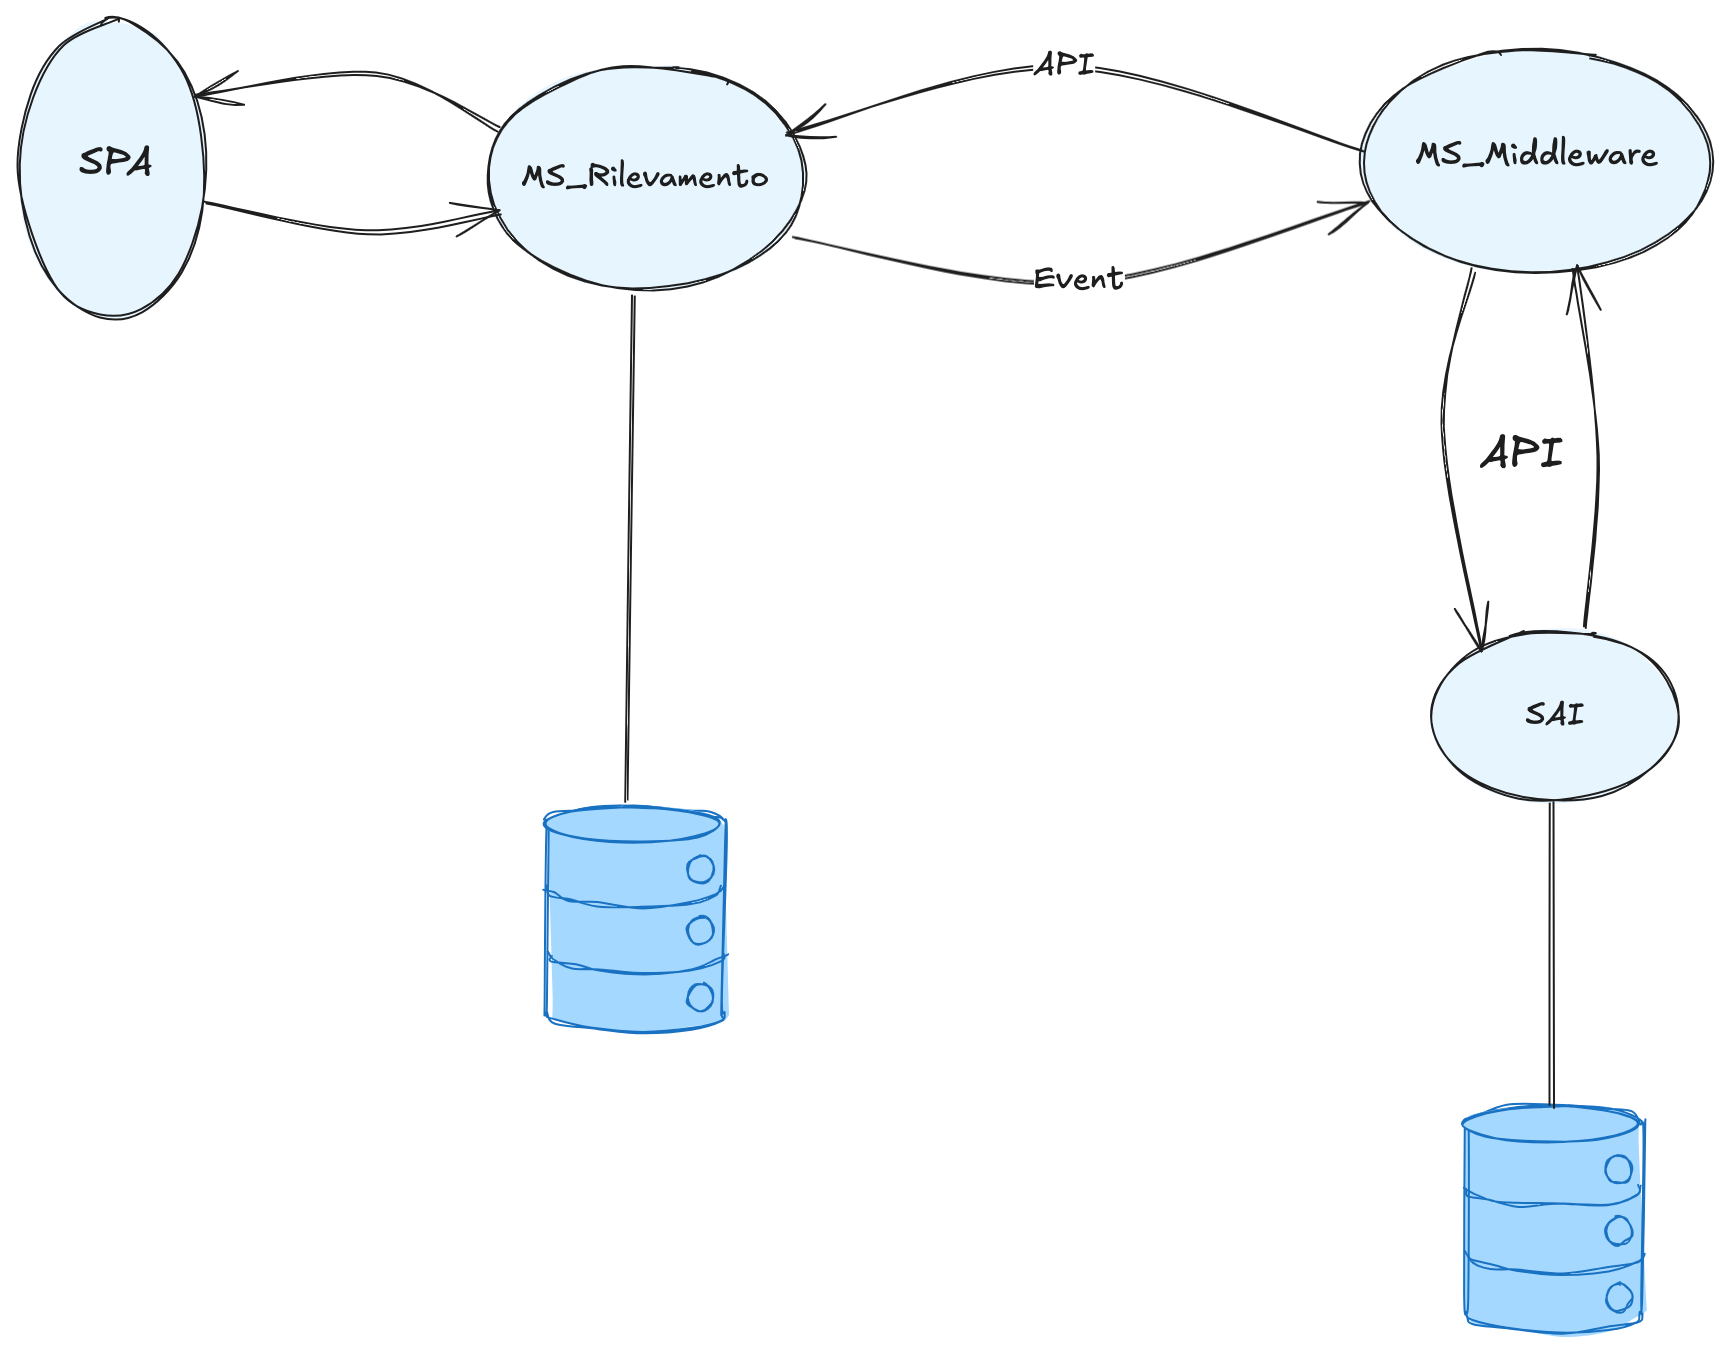
\includegraphics[width=0.6\linewidth]{BCS-Tessi//images/Progettazione.png}
            \caption[Progettazione per l'estrazione del microservizio]{Attività di progettazione per quanto concerne l'estrazione di \texttt{MS\_Rilevamento}}
            \label{fig:progettazione}
        \end{figure}

        \vspace{0.2 em}
        \noindent Date le dimensioni molto grandi del monolite in esame, l'azienda ha scelto di optare per una migrazione graduale. La soluzione più ragionevole è risultata dunque quella di applicare il \textit{pattern} \textit{Anti-Corruption Layer} (ACL) prevedendo la lunga convivenza del monolite e del nuovo sistema a microservizi. In questo caso questo \textit{pattern} trova rappresentazione in \texttt{MS\_Middleware}.

        \vspace{0.2 em}
        \noindent Un altro \textit{pattern} che ho proposto è il \textit{Change Data $Capture_G$}, una tecnica utilizzata per identificare e tracciare le modifiche apportate ai dati in un \textit{database}. Nel nostro caso è utile nei contesti di sincronizzazione tra sistemi eterogenei, ossia di \texttt{MS\_Rilevamento} e di SAI, il monolite. 

        \vspace{0.2em}
        \noindent Per l'implementazione di questo microservizio, insieme al \textit{Product Owner} siamo giunti alla scelta del modello di \textbf{architettura esagonale}, noto anche come \textit{pattern} di porte e adattatori che mira a creare architetture liberamente accoppiate in cui i componenti delle applicazioni possano essere testati in modo indipendente, senza dipendenze da archivi di dati o interfacce utente. Viene utilizzato per isolare la logica aziendale (logica di dominio) dal codice dell'infrastruttura correlato. Le \textbf{porte} sono punti di ingresso indipendenti dalla tecnologia in un componente dell'applicazione. Gli \textbf{adattatori} invece, implementano le interfacce definite dalle porte, consentono una comunicazione fluida tra il nucleo applicativo e i sistemi esterni, facilitando future estensioni o sostituzioni di componenti senza impattare sulla logica di dominio centrale.

        \vspace{0.2 em}
        \noindent Nello specifico abbiamo implementato tutti gli elementi legati al dominio, incluse la dichiarazione degli oggetti e le configurazioni fondamentali in una parte chiamata \textbf{\textit{Core}}. In questo modello, il \textit{Core} include:

        \begin{itemize}
            \item \textbf{modelli di dominio}, che descrivono gli oggetti fondamentali e il loro comportamento, definendo le entità, i \textit{value} \textit{objects} e gli aggregati;
            \item \textbf{servizi di dominio}, che implementano logiche più complesse, mantenendo il dominio autonomo rispetto agli adattatori esterni;
            \item \textbf{eventi di dominio}, che permettono di notificare cambiamenti interni senza creare un forte accoppiamento tra componenti;
            \item \textbf{\textit{application services}}, che rappresentano le operazioni principali eseguibili dall'applicazione, orchestrando l'interazione tra il dominio e le interfacce esterne.
        \end{itemize}

        \vspace{0.2 em}
        \noindent L'altra componente è la \textit{\textbf{Infrastructure}}, che contiene tutti gli elementi necessari per connettere il dominio con il mondo esterno. Questa parte dell'architettura comprende le porte e gli adattatori, nonché i protocolli di comunicazione che permettono l'integrazione tra le varie componenti del sistema, consentendo al \textit{Core} di rimanere isolato e indipendente. Nello specifico, la componente \textit{Infrastructure} comprende:

        \begin{itemize}
            \item \textbf{adattatori di persistenza}: gestiscono l'interazione con il \textit{database}, fornendo meccanismi per il salvataggio e il recupero dei dati senza esporre dettagli implementativi al dominio. Questo può includere \textit{repository} che implementano interfacce definite nel \textit{Core}, consentendo di cambiare la tecnologia di persistenza senza modificare la logica applicativa;
            \item \textbf{adattatori di comunicazione} (API REST, messaggistica): consentono al microservizio di esporre e ricevere dati attraverso protocolli standard come REST (HTTP) o eventi asincroni (message brokers o RabbitMQ). In particolare, le operazioni \texttt{PUT}, \texttt{POST}, \texttt{GET} e \texttt{DELETE} implementano le azioni previste dai casi d'uso del dominio;
            \item \textbf{Web API}: rappresenta il punto di accesso del microservizio, consentendo la comunicazione con altri servizi, come il \textit{Middleware} o il monolite esistente. Questa API traduce le richieste esterne in comandi eseguibili dal \textit{Core} e restituisce le risposte formattate in un protocollo standard ($JSON_G$, approfondito nella sezione successiva);
        \end{itemize}

        \vspace{0.2 em}
        \noindent Questa suddivisione consente di ottenere un sistema modulare, scalabile e manutenibile, in cui il dominio rimane indipendente dai dettagli tecnologici. Inoltre, la \textit{Infrastructure} può essere sostituita o aggiornata senza impattare direttamente il \textit{Core}, rendendo il sistema più flessibile nel tempo. Una buona rappresentazione dei risultati della progettazione è osservabile nella Figura \ref{fig:esagonale}. 
        
        \begin{figure}[H]
            \centering
            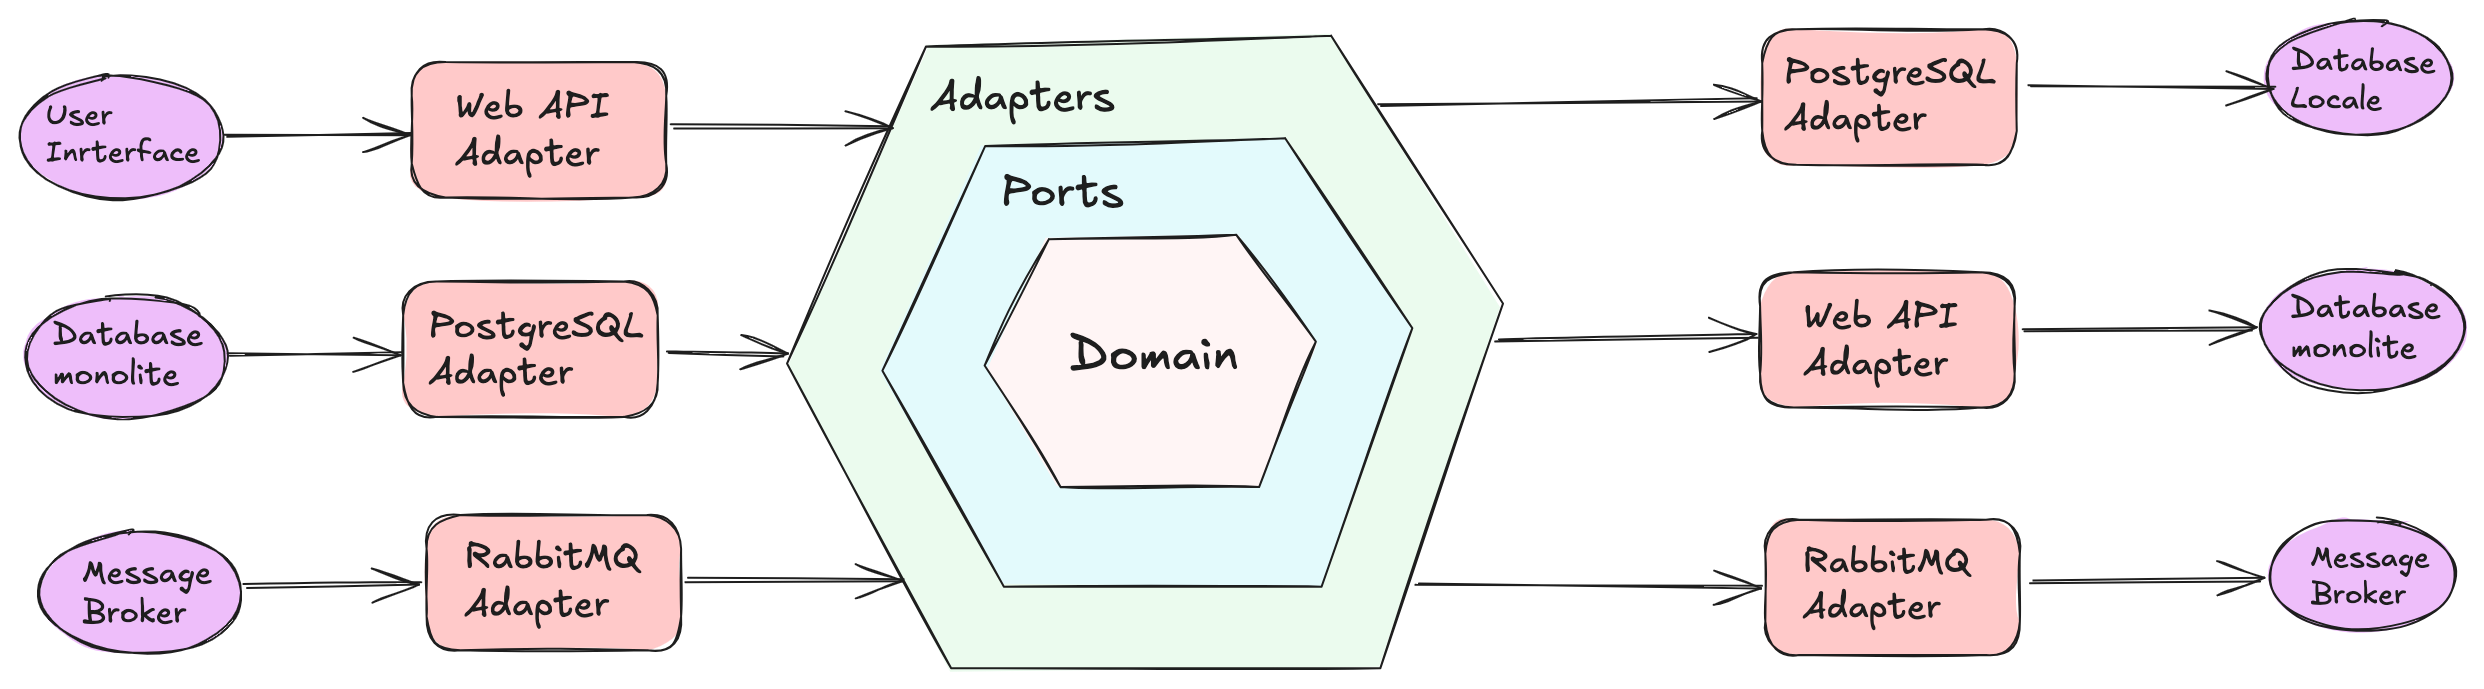
\includegraphics[width=1\linewidth]{BCS-Tessi//images/esagonale.png}
            \caption[Rappresentazione dell'architettura esagonale]{Rappresentazione grafica dell'architettura esagonale e i rispettivi adattatori e porte.}
            \label{fig:esagonale}
        \end{figure}


        \vspace{0.2 em}
        \noindent Come anticipato nella precedente sezione, un problema da risolvere è quello di effettuare due letture sul \textit{bounded context} \texttt{Lavorazione}. La soluzione trovata per fare ciò è effettuare una lettura su \texttt{MS\_Rilevamento} tramite un \textit{adapter} PostgreSQL sul \textit{database} locale, e una su SAI tramite una connessione PostgreSQL al \textit{database} del monolite stesso, strategia sempre visibile nella Figura \ref{fig:esagonale}. 
        
        \vspace{0.2 em}
        \noindent Per la scrittura sui \textit{database} invece, studiando i \textit{pattern} di scomposizione per questa specifica situazione ho individuato il \textit{pattern} \textbf{\textit{Database Wrapping Service}}\footnote{S. Newman, Monolith to Microservices: Evolutionary Patterns to Transform Your Monolith, O'Reilly Media, 2019}. Nello specifico si implementa un servizio intermedio (\textit{wrapping service}) che si occupa di esporre le informazioni di SAI tramite delle \textit{Web} API senza esporre direttamente il \textit{database} sottostante, il tutto sempre riconducibile alla Figura \ref{fig:esagonale}. 

        \vspace{0.2 em}
        \noindent In questo modo, il \textit{team} che gestisce il monolite è responsabile dell' aggiornamento delle API in caso di modifiche alla struttura del \textit{database}, e il \textit{team} di \texttt{MS\_Rilevamento} non deve preoccuparsi dei cambiamenti interni a SAI. Questo approccio riduce l'accoppiamento tra i sistemi, rendendo più facile l'evoluzione della struttura dei dati.

        \vspace{0.2 em}
        \noindent Infine, insieme al \textit{Product Owner}, abbiamo pensato a come sincronizzare questi dati. Dallo studio della letteratura sui \textit{pattern} è emerso come migliore per il nostro problema il \textit{\textbf{Change Data Capture}} \textbf{(CDC)} implementato con un \textbf{\textit{Batch Delta Copier}}\ap{2}. 
        
        
        \vspace{0.2 em} 
        \noindent Il \textit{Change Data Capture} è un \textit{pattern} che monitora e cattura le modifiche ai dati in un sistema di origine (nel nostro caso SAI) per sincronizzarle con sistemi di destinazione, garantendo così la coerenza delle informazioni attraverso piattaforme diverse. Il \textit{Batch Delta Copier} è un'implementazione specifica di CDC che funziona identificando periodicamente i dati nuovi o modificati dalla sorgente (il \textit{delta}) e copiandoli in blocco verso la destinazione durante finestre temporali programmate. Nel nostro caso è un sistema basato sui \textit{transaction log}: quando una nuova transazione arriva nel \textit{database} del microservizio, viene registrata in un file di \textit{log} senza impattare il monolite. È quindi possibile rilevare tali modifiche e trasferirle dal \textit{log} a SAI. Una rappresentazione grafica di questo processo si può osservare nella Figura.

        \begin{figure}[H]
            \centering
            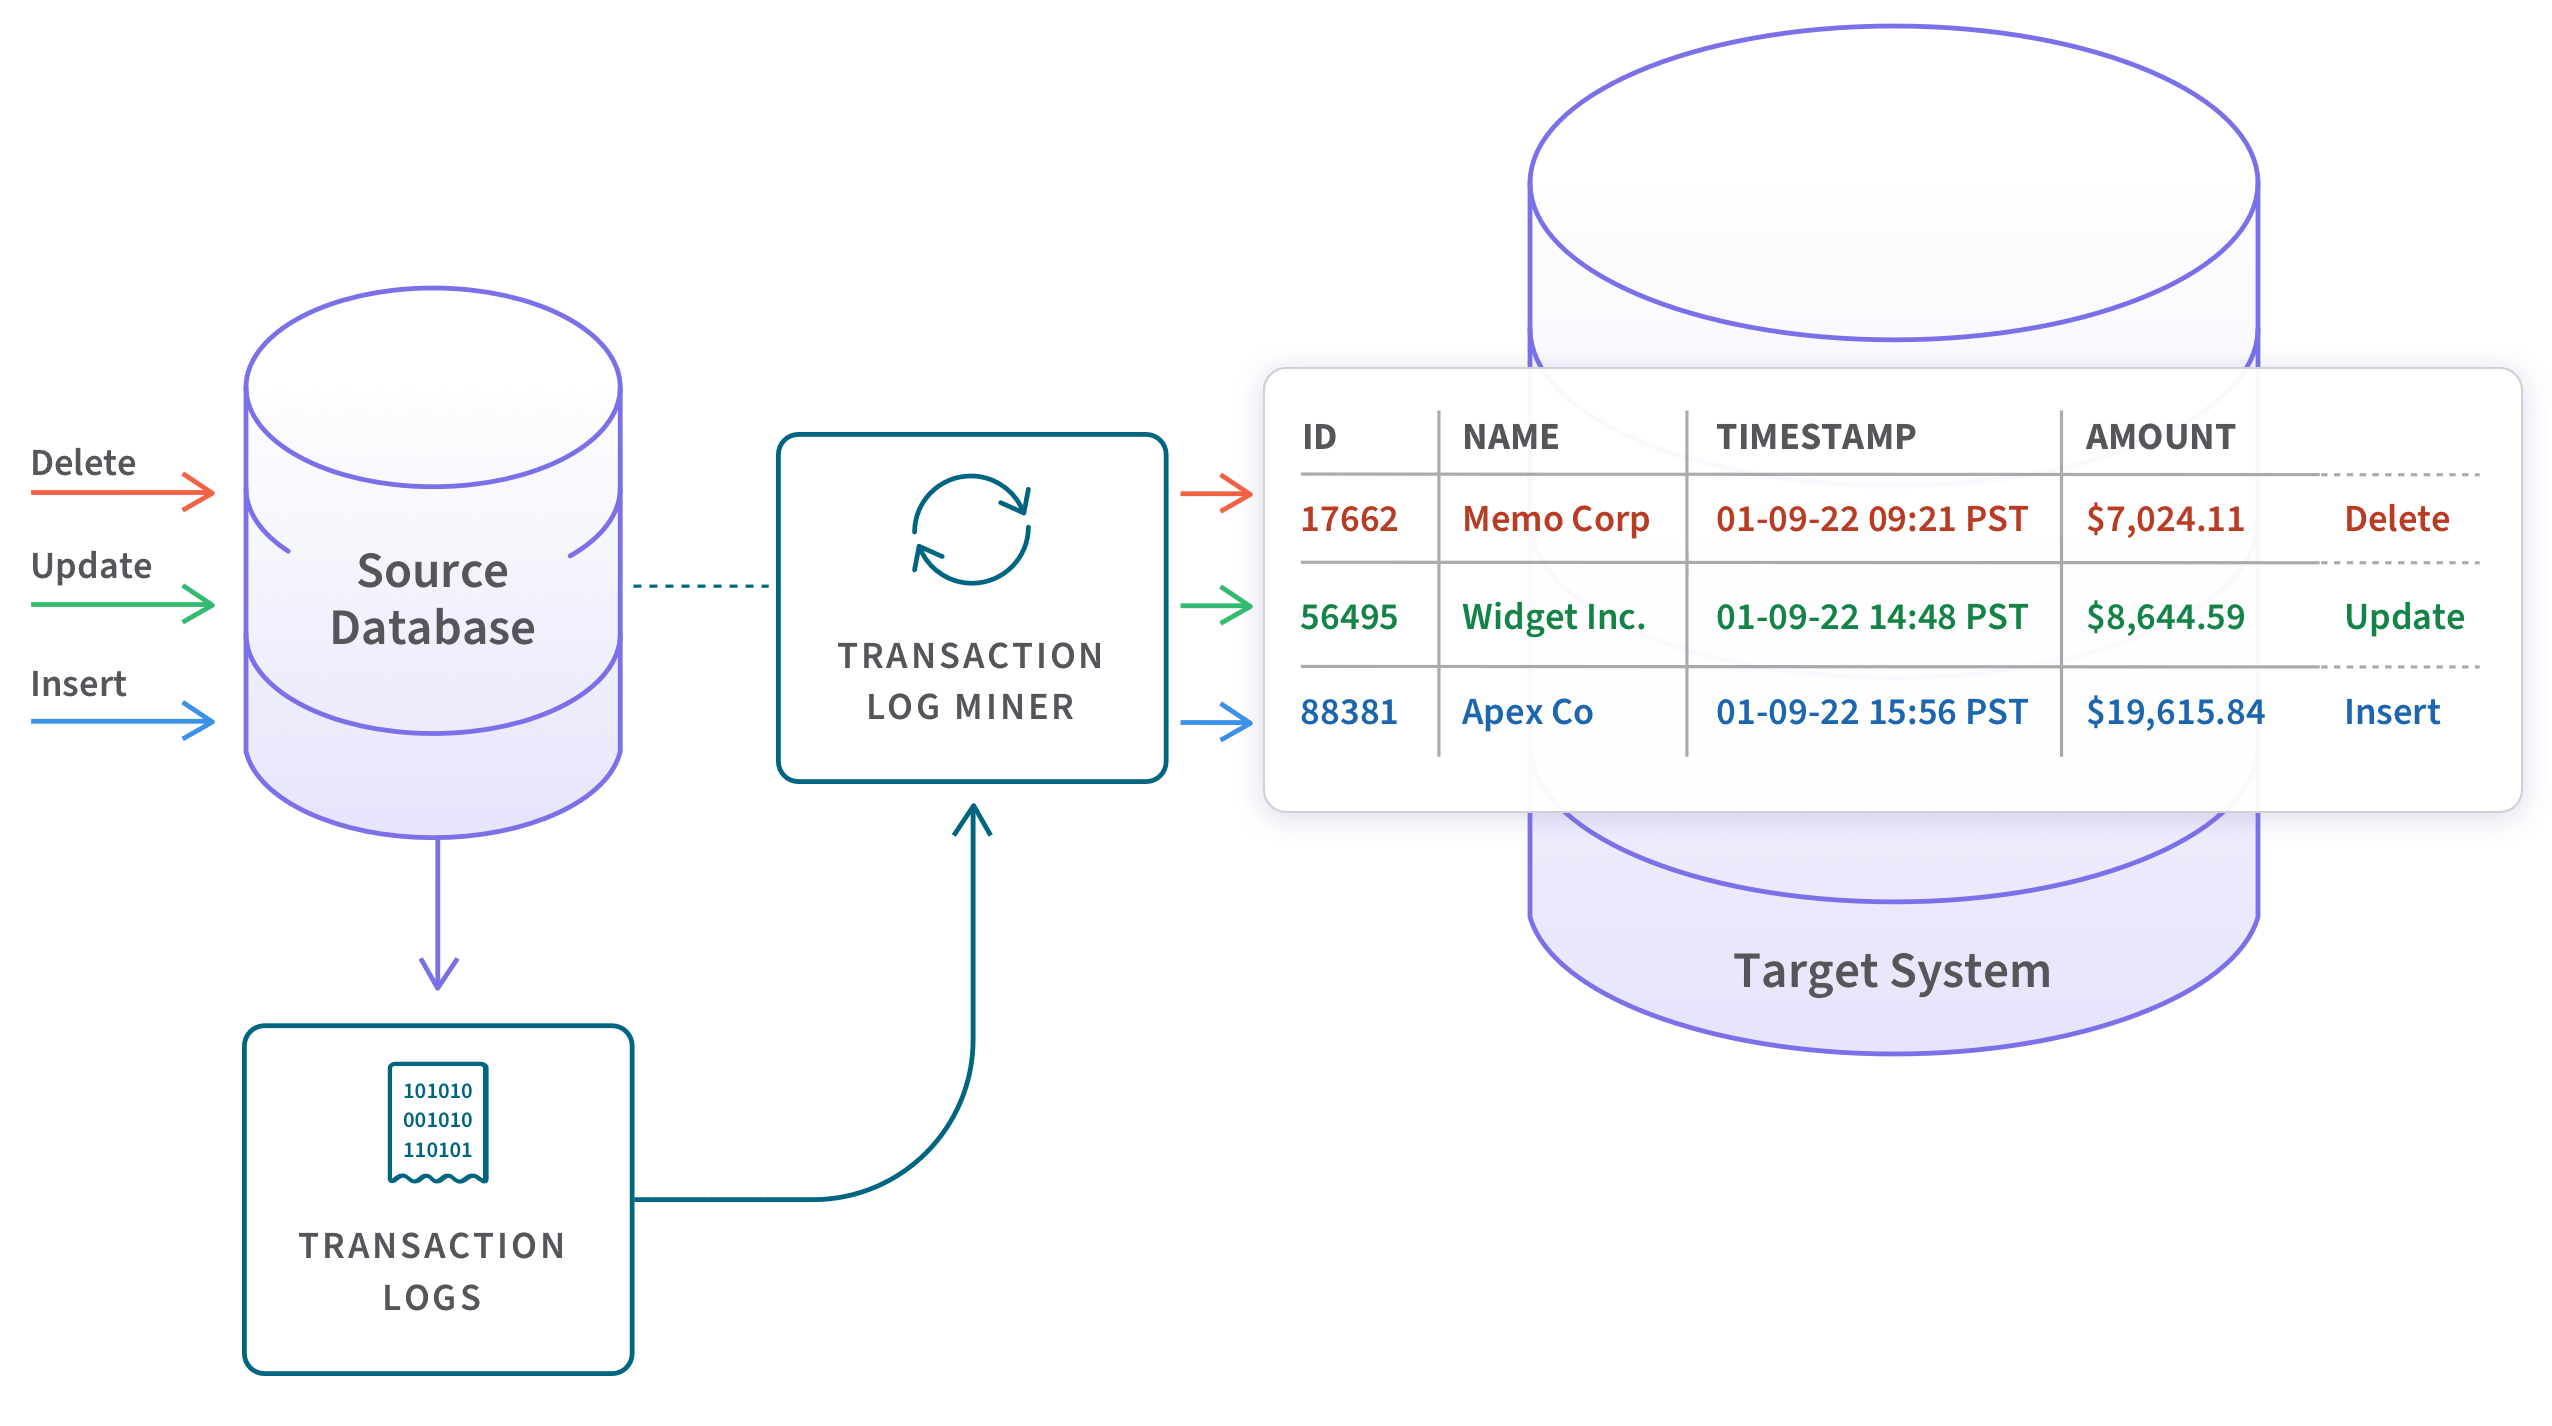
\includegraphics[width=1\linewidth]{BCS-Tessi//images/cdc.png}
            \caption[Schema del \textit{pattern} \textit{Change Data Capture}]{Rappresentazione del \textit{pattern} \textit{Change Data Capture} (CDC) nel contesto dell'attività di progettazione. Fonte: \href{https://www.qlik.com/us/change-data-capture/cdc-change-data-capture}{https://www.qlik.com/us/change-data-capture/cdc-change-data-capture} \textit{(ultima visita: 29/03/2025)}}
            \label{fig:cdc}
        \end{figure}

        \vspace{0.2 em}
        \noindent Le attività di progettazione, oltre ad avermi consentito di individuare i \textit{pattern} da utilizzare, hanno permesso a me e al \textit{Product Owner} di definire una serie di metriche interessanti per questo progetto. L'obiettivo primario è stato valutare e monitorare delle prestazioni dell'applicazione prima e dopo lo sviluppo del microservizio.

        \vspace{0.2 em}
        \noindent Inizialmente, abbiamo proceduto alla costruzione di un \textit{Product Backlog} dettagliato, approfondito nella Sezione 1.4. Non mi sono limitata a catalogare i requisiti, ma li ho anche associati a stime temporali indicative, consentendomi una pianificazione più accurata, tutto sempre con la supervisione e consiglio del \textit{Product Owner}. Tale strumento mi ha fornito una proiezione affidabile dei tempi necessari per l'implementazione di ciascun componente del progetto. 
        In particolare, la previsione temporale che ho svolto rispetto ai requisiti individuati mi ha permesso di stimare un completamento del 73\% dei requisiti totali contenuti nel \textit{Product Backlog}. La Figura \ref{fig:product-backlog} presenta una rappresentazione visiva del grado di copertura previsto. 

        \begin{figure}[H]
            \centering
            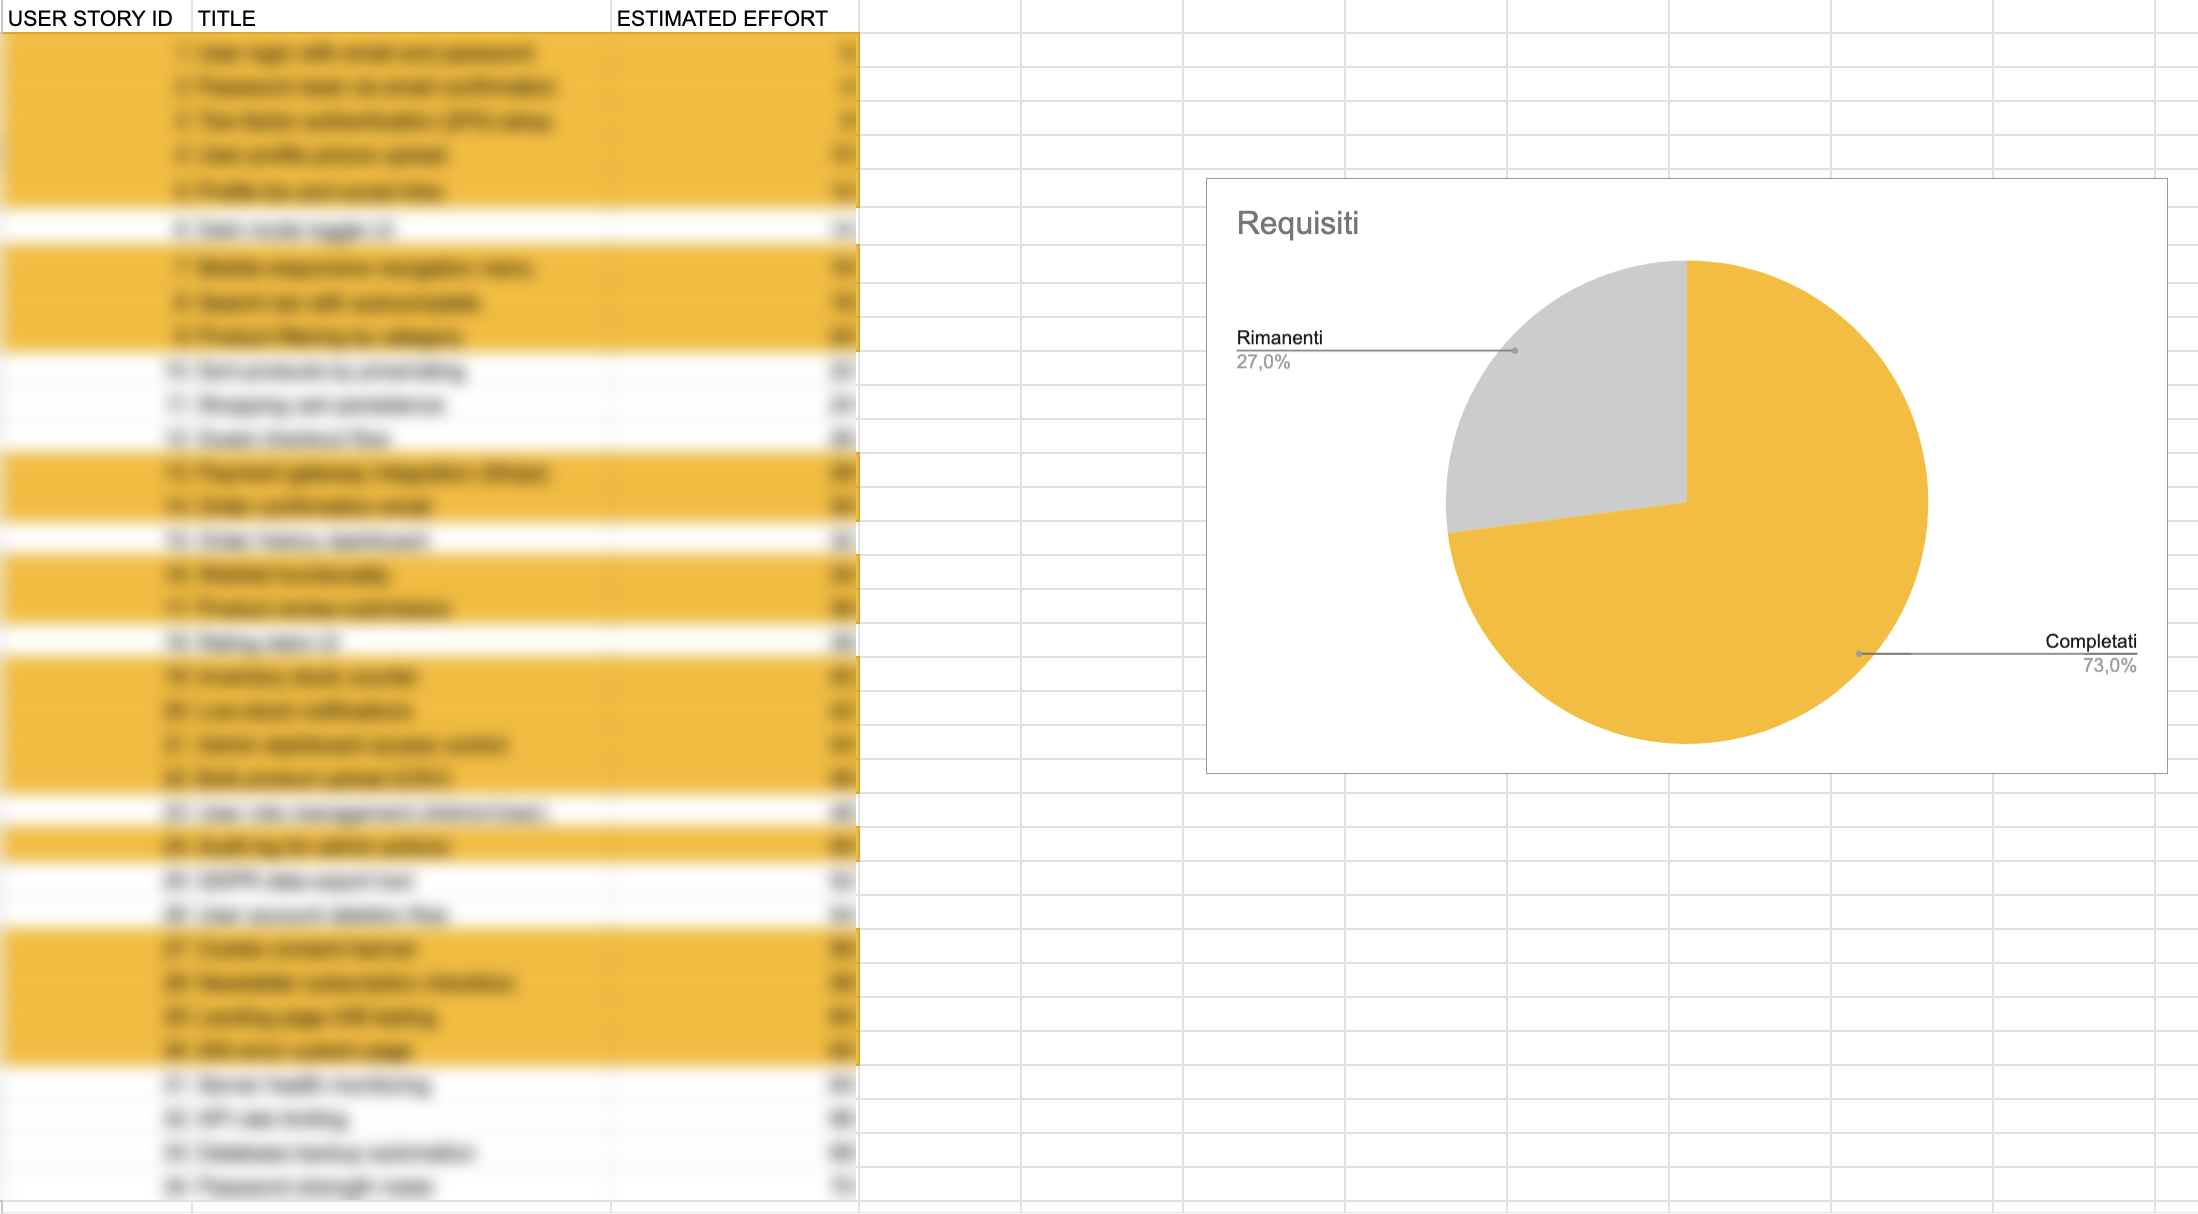
\includegraphics[width=0.7\linewidth]{BCS-Tessi//images/metriche.png}
            \caption[\textit{Product Backlog} e delle metriche]{\textit{Product Backlog} utilizzato durante il processo di progettazione, accompagnato dal una misura della quantità di requisiti che le soluzioni trovate potranno soddisfare.}
            \label{fig:product-backlog}
        \end{figure}

        \vspace{0.2 em}
        \noindent Un aspetto particolarmente significativo dell'analisi è stata la misurazione delle prestazioni del sistema esistente. Abbiamo effettuato una valutazione delle velocità di estrazione dati nel sistema monolitico preesistente, predisponendo un \textit{benchmark} essenziale per le successive comparazioni. Questo approccio ha gettato le basi per una valutazione oggettiva dei miglioramenti prestazionali introdotti dal nuovo servizio.

        \vspace{0.2 em}
        \noindent L'analisi si è poi estesa a considerazioni economiche più ampie, introducendo il concetto di \textit{Return On $Investment_G$} ($ROI_G$). Tale prospettiva ha rivelato la complessità intrinseca della trasformazione architetturale: l'estrazione di un microservizio comporta investimenti iniziali significativi in termini di risorse, formazione e sviluppo. La validità dell'intervento dipende quindi dalla capacità di generare un vantaggio tangibile per l'organizzazione.

        \vspace{0.2 em}
        \noindent Abbiamo quindi proceduto a una misurazione comprensiva delle metriche di \textit{performance}, analizzando la velocità dei processi interni nel sistema corrente. Questo approccio metodologico ha predisposto un solido \textit{framework} per le successive attività di validazione, permettendo un confronto tra le prestazioni del sistema monolitico e la nuova soluzione implementata.

        
        \subsection{Implementazione}
        Le attività di progettazione sono state senza dubbio le più complesse, soprattutto a causa della mancanza di soluzioni definitive e della relativa novità del concetto di migrazione verso i microservizi\footnote{D. Shadija, M. Rezai, and R. Hill, "Towards an Understanding of Microservices," in Proceedings of the 2017 IEEE International Conference on Computer and Information Technology (CIT), Helsinki, Finland, 2017, pp. 1072-1078}. Nonostante le difficoltà iniziali, una volta definita la strategia da adottare, l'implementazione è proseguita in modo naturale, seguendo il percorso tracciato.  

        \vspace{0.2 em}
        \noindent L'attività di codifica è stata improntata su un approccio \textit{learn by doing}: pur avendo una base di riferimento, ho dovuto affinare le mie competenze sul campo, confrontandomi regolarmente con il \textit{tutor} aziendale e il \textit{Product Owner} per ricevere \textit{feedback} e indicazioni utili.
        
        \noindent Nello specifico, ho potuto implementare una struttura di progetto molto precisa, già anticipata nella Sezione 3.2.2 e rappresentata nella Figura \ref{fig:code-structure}.

         
        \begin{figure}[H]
            \centering
            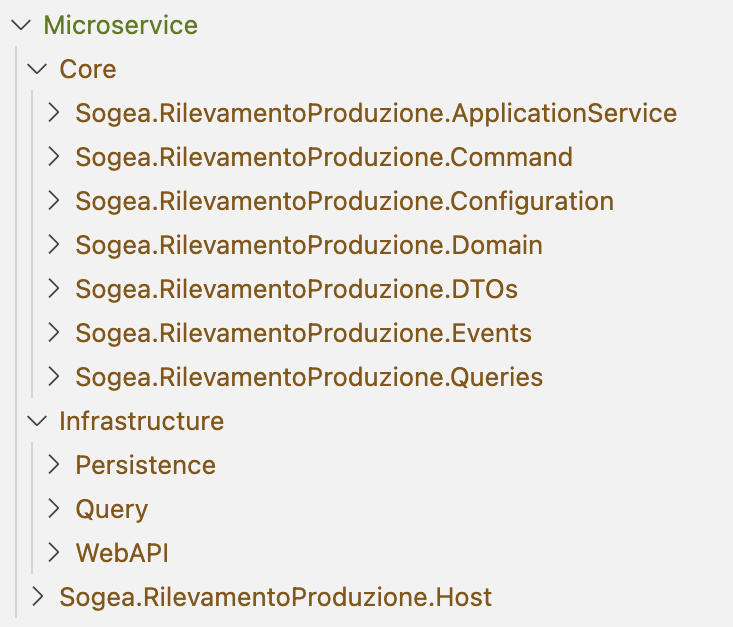
\includegraphics[width=0.5\linewidth]{BCS-Tessi//images/dev_tree.png}
            \caption{Struttura del codice utilizzata per l'estrazione del microservizio.}
            \label{fig:code-structure}
        \end{figure}

        \vspace{0.2 em}
        \noindent Analizzando più approfonditamente la struttura del microservizio \texttt{Sogea.Rilevamento} \\
        \noindent \texttt{Produzione}, posso espandere diversi concetti architetturali, descritti come segue. 
            \subsubsection{Domain-Driven Design (DDD)}
            Tutto ruota attorno al progetto \texttt{Sogea.}\texttt{Rilevamento}  \texttt{Produzione.}\texttt{Domain}, che è il cuore dell'applicazione. Qui ci sono entità, aggregati e \textit{value objects}, regole di \textit{business} e tutta la logica che descrive cosa significa \texttt{Rilevamento} \texttt{Produzione} per l'azienda. È isolato dal \textit{database}, dalle API e da dettagli tecnici, proprio come DDD suggerisce. L'immagine \ref{fig:rilevamento-aggregate} racconta un esempio di entità (\texttt{Rilevamento}) all'interno di un aggregato (\texttt{Lavorazione}\texttt{Aggregate}). Sono implementati nello specifico i metodi \texttt{Inizia}\texttt{Rilevamento} e \texttt{Registra}\texttt{Rilevamento}. 

            \begin{figure}[H]
                \centering
                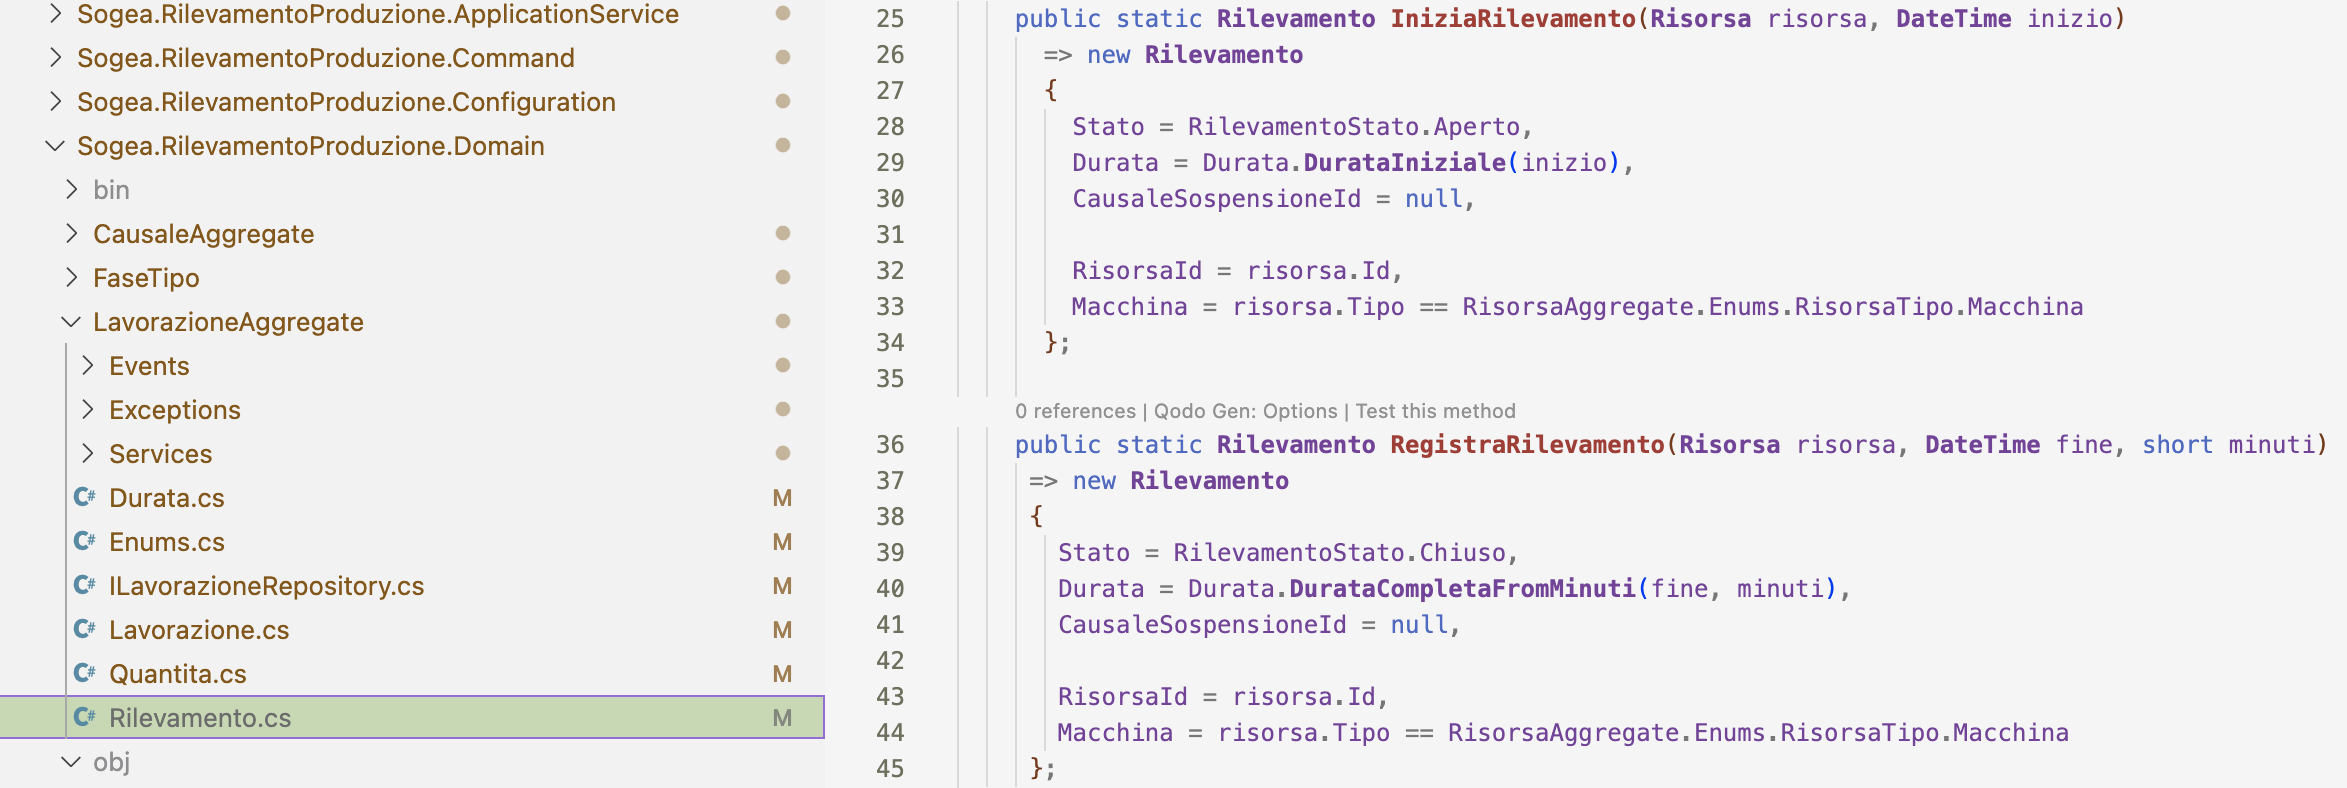
\includegraphics[width=1\linewidth]{BCS-Tessi//images/rilevamento_aggregate.png}
                \caption[Definizione dei metodi di \texttt{Rilevamento}]{Definizione dei metodi dell'entità \texttt{Rilevamento} all'interno dell'aggregato \texttt{LavorazioneAggregate}.}
                \label{fig:rilevamento-aggregate}
            \end{figure}
            
            \subsubsection{Command Query Responsibility Segregation (CQRS)}
            Il \textit{Command Query Responsibility $Segregation_G$} è un \textit{pattern} che divide il sistema in due parti: i \texttt{Command}, che gestiscono le modifiche ai dati, e le \texttt{Query}, che si occupano delle letture. Questa separazione è un'applicazione pratica caratteristica del CQRS, approccio particolarmente utile nel \textit{Domain-Driven Design} per affrontare scenari complessi garantendo maggiore scalabilità. In questo contesto, gli \texttt{ApplicationService} svolgono un ruolo cruciale di coordinamento, poiché racchiudono la logica delle \textit{user story} mantenendo il dominio pulito da contaminazioni esterne. Questa struttura permette di gestire in modo più efficace e organizzato le diverse responsabilità all'interno del sistema.

            \vspace{0.2 em}
            \noindent Gli $handler_G$ sono il cuore del CQRS in questo sistema. Nello specifico gli \textit{handler} dei comandi ricevono richieste di modifica, le validano, applicano la logica di dominio e ne aggiornano lo stato. Gli \textit{handler} delle $query_G$ invece, ricevono richieste di informazioni e restituiscono i dati necessari senza modificare lo stato. Un esempio rappresentativo di un hanler è raccontato dalla Figura \ref{fig:handler}, in cui si può osservare un esempio dell'handler \texttt{Resource}\texttt{Handler}, il quale implementa i comandi \texttt{Get}, \texttt{Create}, \texttt{Delete}, secondo il protocollo REST basato su HTTP. Questo definisce un insieme di vincoli e proprietà per la creazione di servizi \textit{web}, già citato nella Sezione 1.7. Nell'implementazione mostrata, il \texttt{Resource}\texttt{Handler} fornisce un'interfaccia conforme ai principi REST, esponendo le operazioni fondamentali per la manipolazione delle risorse attraverso i metodi standard HTTP. In questo caso, rispettivamente all'ordine di apparizione nell'immagine, \textit{read}, \textit{create}, \textit{delete}. 

            \begin{figure}[H]
                \centering
                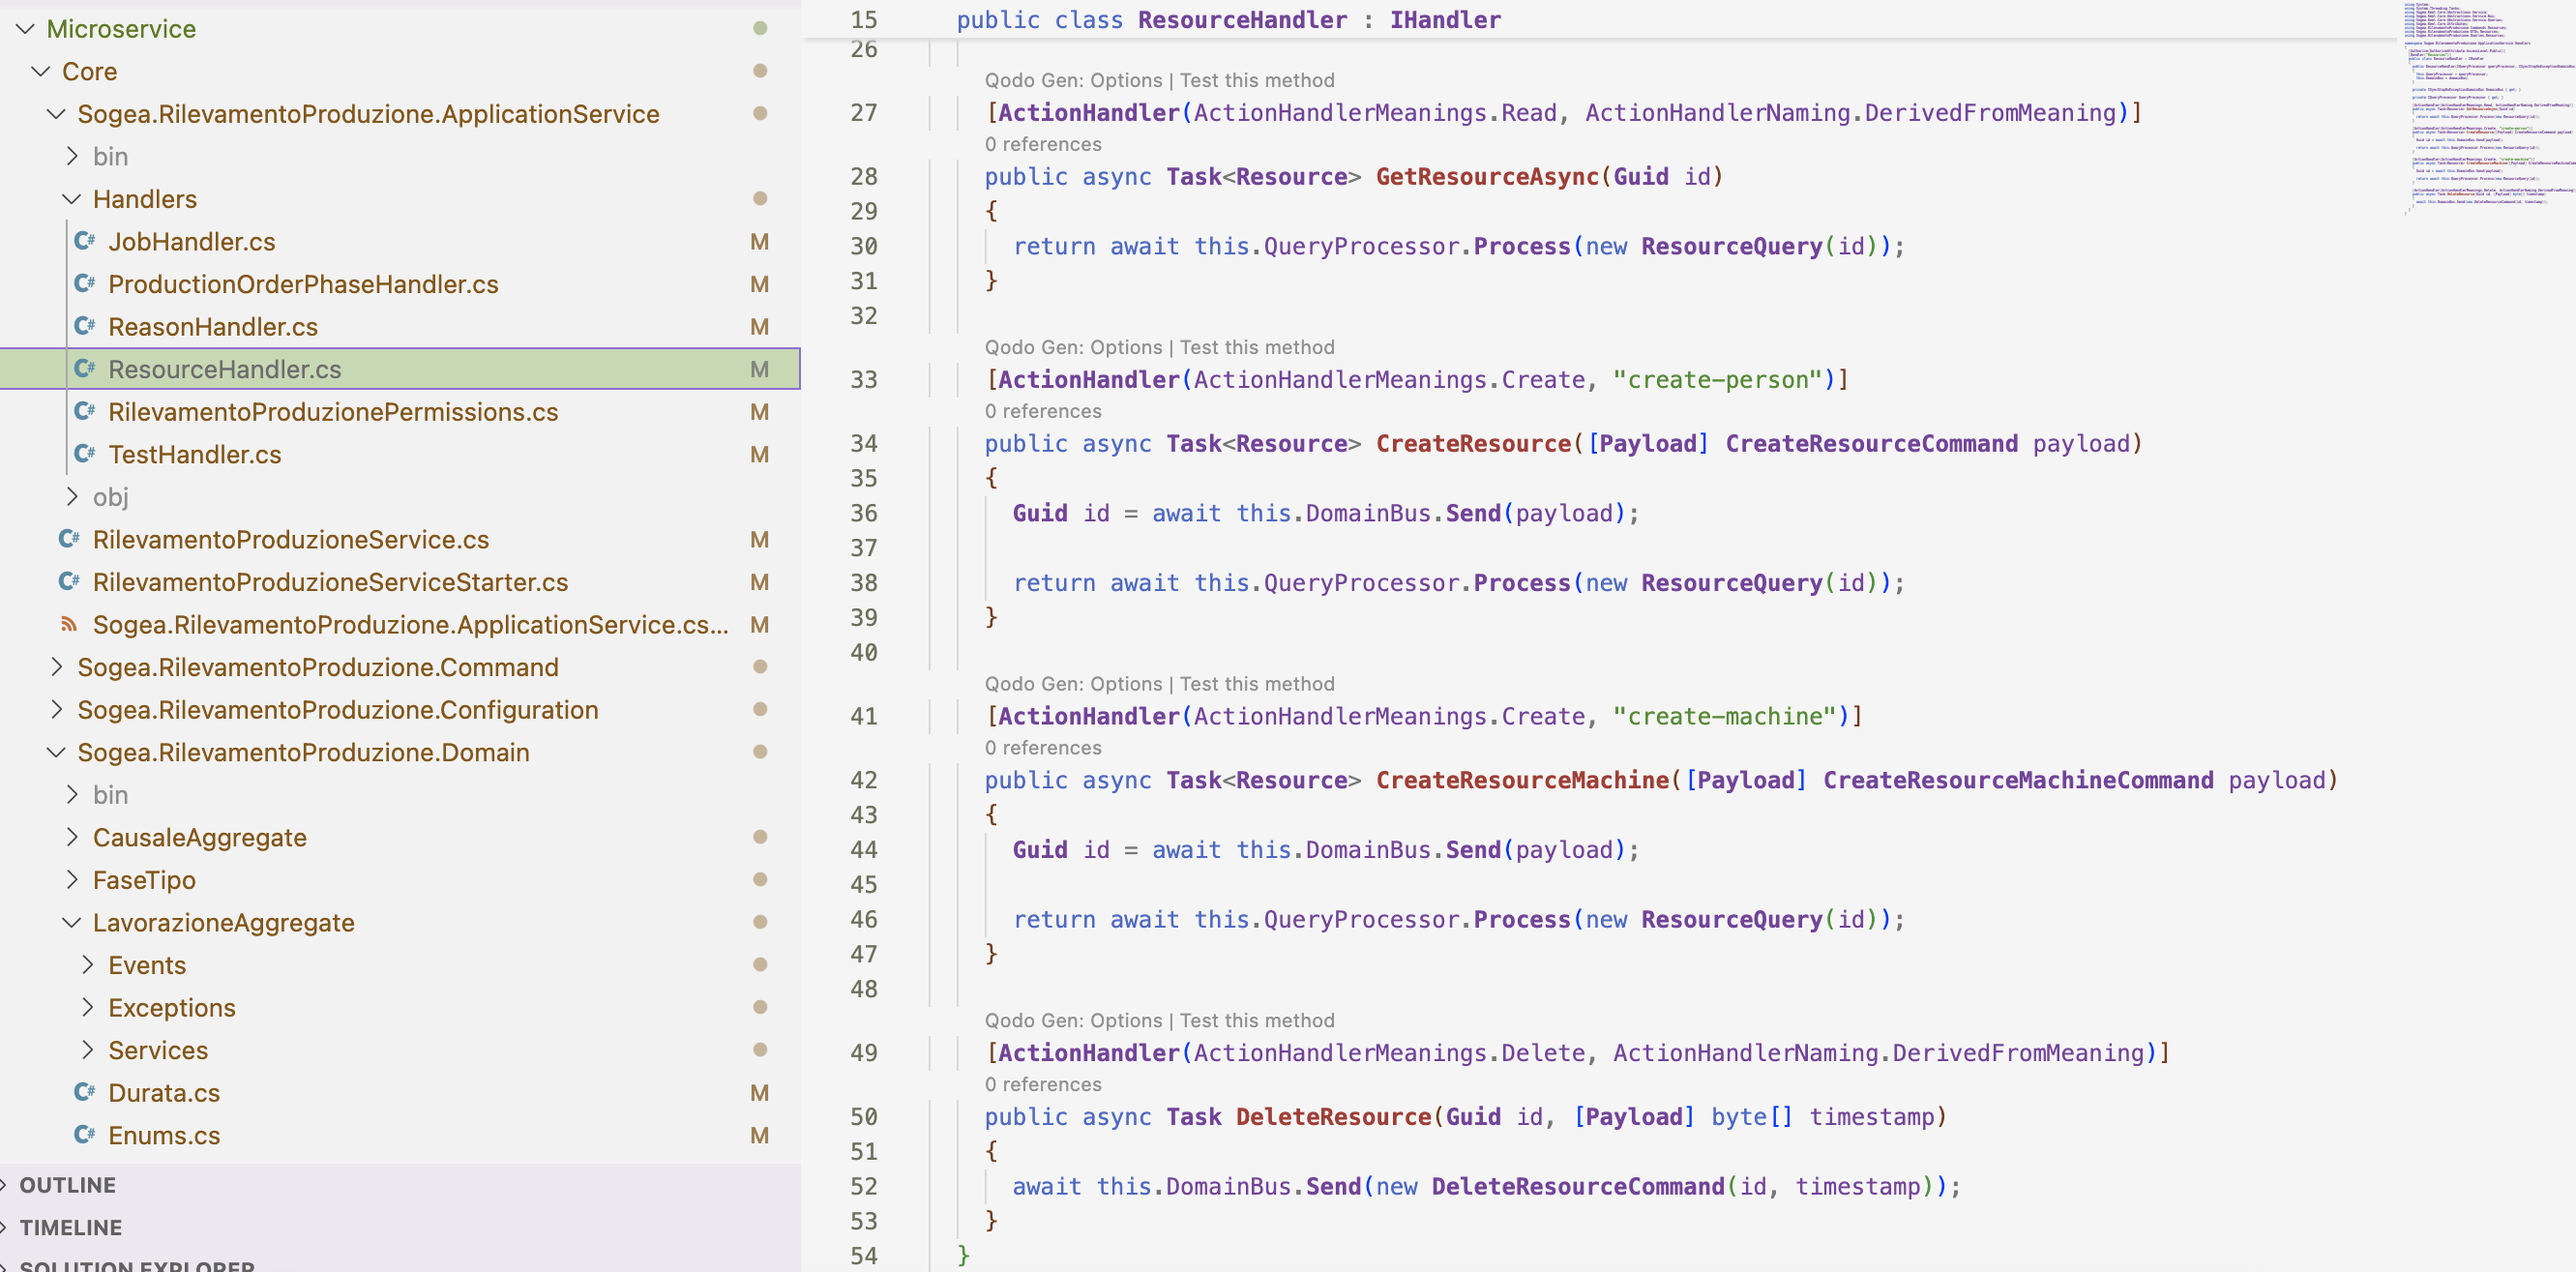
\includegraphics[width=1\linewidth]{BCS-Tessi//images/handler_cmd_dto.png}
                \caption[Implementazione di \texttt{ResourceHandler} e i rispettivi metodi.]{Il \texttt{ResourceHandler} implementa le operazioni per la creazione, lettura e cancellazione dei dati seguendo i principi REST, fungendo da interfaccia tra le richieste HTTP e la logica applicativa del sistema di \texttt{Rilevamento}\texttt{Produzione}.}
                \label{fig:handler}
            \end{figure}

            \vspace{0.2 em}
            \noindent Sempre nella Figura \ref{fig:handler}, si osserva la parola chiave \texttt{payload}. In questo caso \texttt{payload} svolge un ruolo fondamentale come contenitore di dati per le operazioni di creazione delle risorse. Questo è un attributo che indica che il parametro contiene i dati necessari per l'operazione di creazione. Quando una richiesta di creazione arriva al \textit{handler}, il \texttt{payload} contiene tutte le informazioni necessarie fornite dal \textit{client} (come proprietà, valori e configurazioni della risorsa da creare). Questo viene poi inoltrato al \texttt{DomainBus} attraverso il metodo \texttt{Send()}, che lo trasmette al livello di dominio appropriato per l'elaborazione. 

            \vspace{0.2 em}
            \noindent Questo \texttt{payload} corrisponde a un \textit{Data Transfer Object}, ossia un oggetto usato per trasferire dati tra sistemi o livelli di un'applicazione, senza contenere logica di \textit{business}. Serve a ottimizzare la comunicazione e ridurre il numero di chiamate tra componenti. È un \texttt{payload} perché rappresenta il contenuto effettivo trasmesso in una richiesta o risposta. 

            
            \subsubsection{Data Transfer Object (DTO)}
            I \textit{Data Transfer $Objects_G$ } (DTO$s_G$) sono rilevanti in questo contesto perché permette di disaccoppiare il modello di dominio delle interfacce esterne e fornisce anche una struttura chiara per i dati in ingresso e in uscita, senza esporre dettagli implementativi interni. 

            \vspace{0.2 em}
            \noindent Come anticipato nel paragrafo precedente, quando un \textit{client} invia una richiesta, utilizza un DTO come \textbf{$payload_G$}, ossia la parte di un messaggio o di una richiesta che contiene i dati effettivi da elaborare. Questo DTO viene poi elaborato dall'\textit{handler} appropriato che esegue la logica necessaria. I DTO permettono di controllare esattamente quali dati vengono trasferiti, facilitano la validazione e migliorano la sicurezza nascondendo i dettagli implementativi del dominio. Nella Figura \ref{fig:dto} si può osservare un esempio di \texttt{payload}, un DTO che contiene il messaggio con le informazioni che verranno effettivamente mandate al \textit{client} che fa la richiesta. Nel caso specifico, si tratta di un \texttt{rilevamento} rispetto a una \texttt{lavorazione}. 

            \begin{figure}[H]
                \centering
                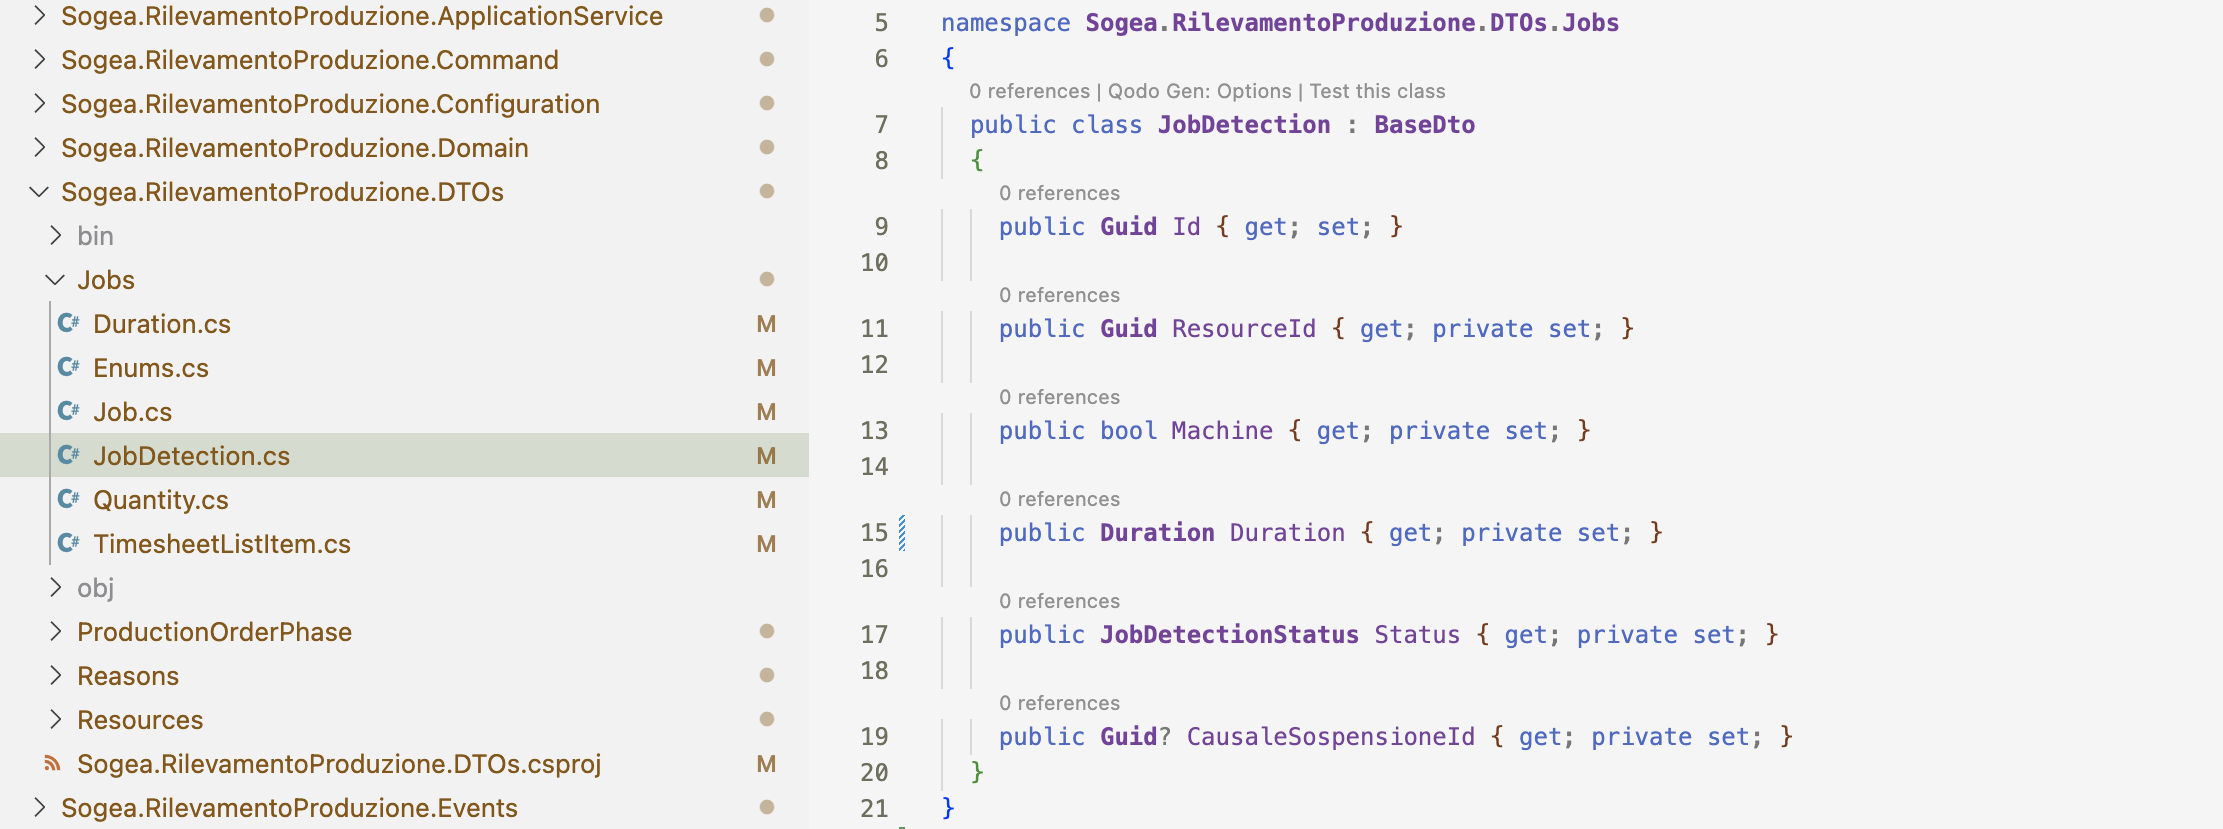
\includegraphics[width=1\linewidth]{BCS-Tessi//images/dto.png}
                \caption{Rappresentazione di un \textit{Data Transfer Object}}
                \label{fig:dto}
            \end{figure}
            
        \noindent In sintesi, in questo microservizio, CQRS con \textit{handler} e DTO offre una separazione chiara delle responsabilità, migliora la manutenibilità del codice e permette di ottimizzare separatamente le operazioni di lettura e scrittura.

        \subsubsection{Web API}
        \vspace{0.2 em}
        \noindent I microservizi, per loro natura intrinseca, comportano significative attività di integrazione per garantire una comunicazione efficace tra i diversi componenti. Un esempio concreto di questa necessità è rappresentato dalla soluzione implementata per il problema, presentato nelle sezioni immediatamente precedenti, della duplice lettura, che si verificava sia sul sistema monolitico sia sul microservizio \texttt{MS\_Rilevamento} da parte di \texttt{OrdineProduzioneFase}. Per risolvere questa criticità, è stata sviluppata un'\textbf{API} dedicata che funge da intermediario nella comunicazione, ottimizzando così il flusso di dati tra le diverse parti dell'architettura.

    
        \vspace{0.2 em}
        \noindent Il componente fondamentale che implementa l'operazione di lettura all'interno dell'API è il metodo \texttt{FindByFaseAsync} della classe \texttt{OrdineProduzioneRepository}. Questo metodo esemplifica l'implementazione di un'operazione di recupero dati secondo il paradigma REST, approfondito nella Sezione 1.7.

        \vspace{0.2 em}
        \noindent L'operazione è raccontata nella Figura \ref{fig:api}, e si articola attraverso i seguenti passaggi.

         \begin{figure}[H]
            \centering
            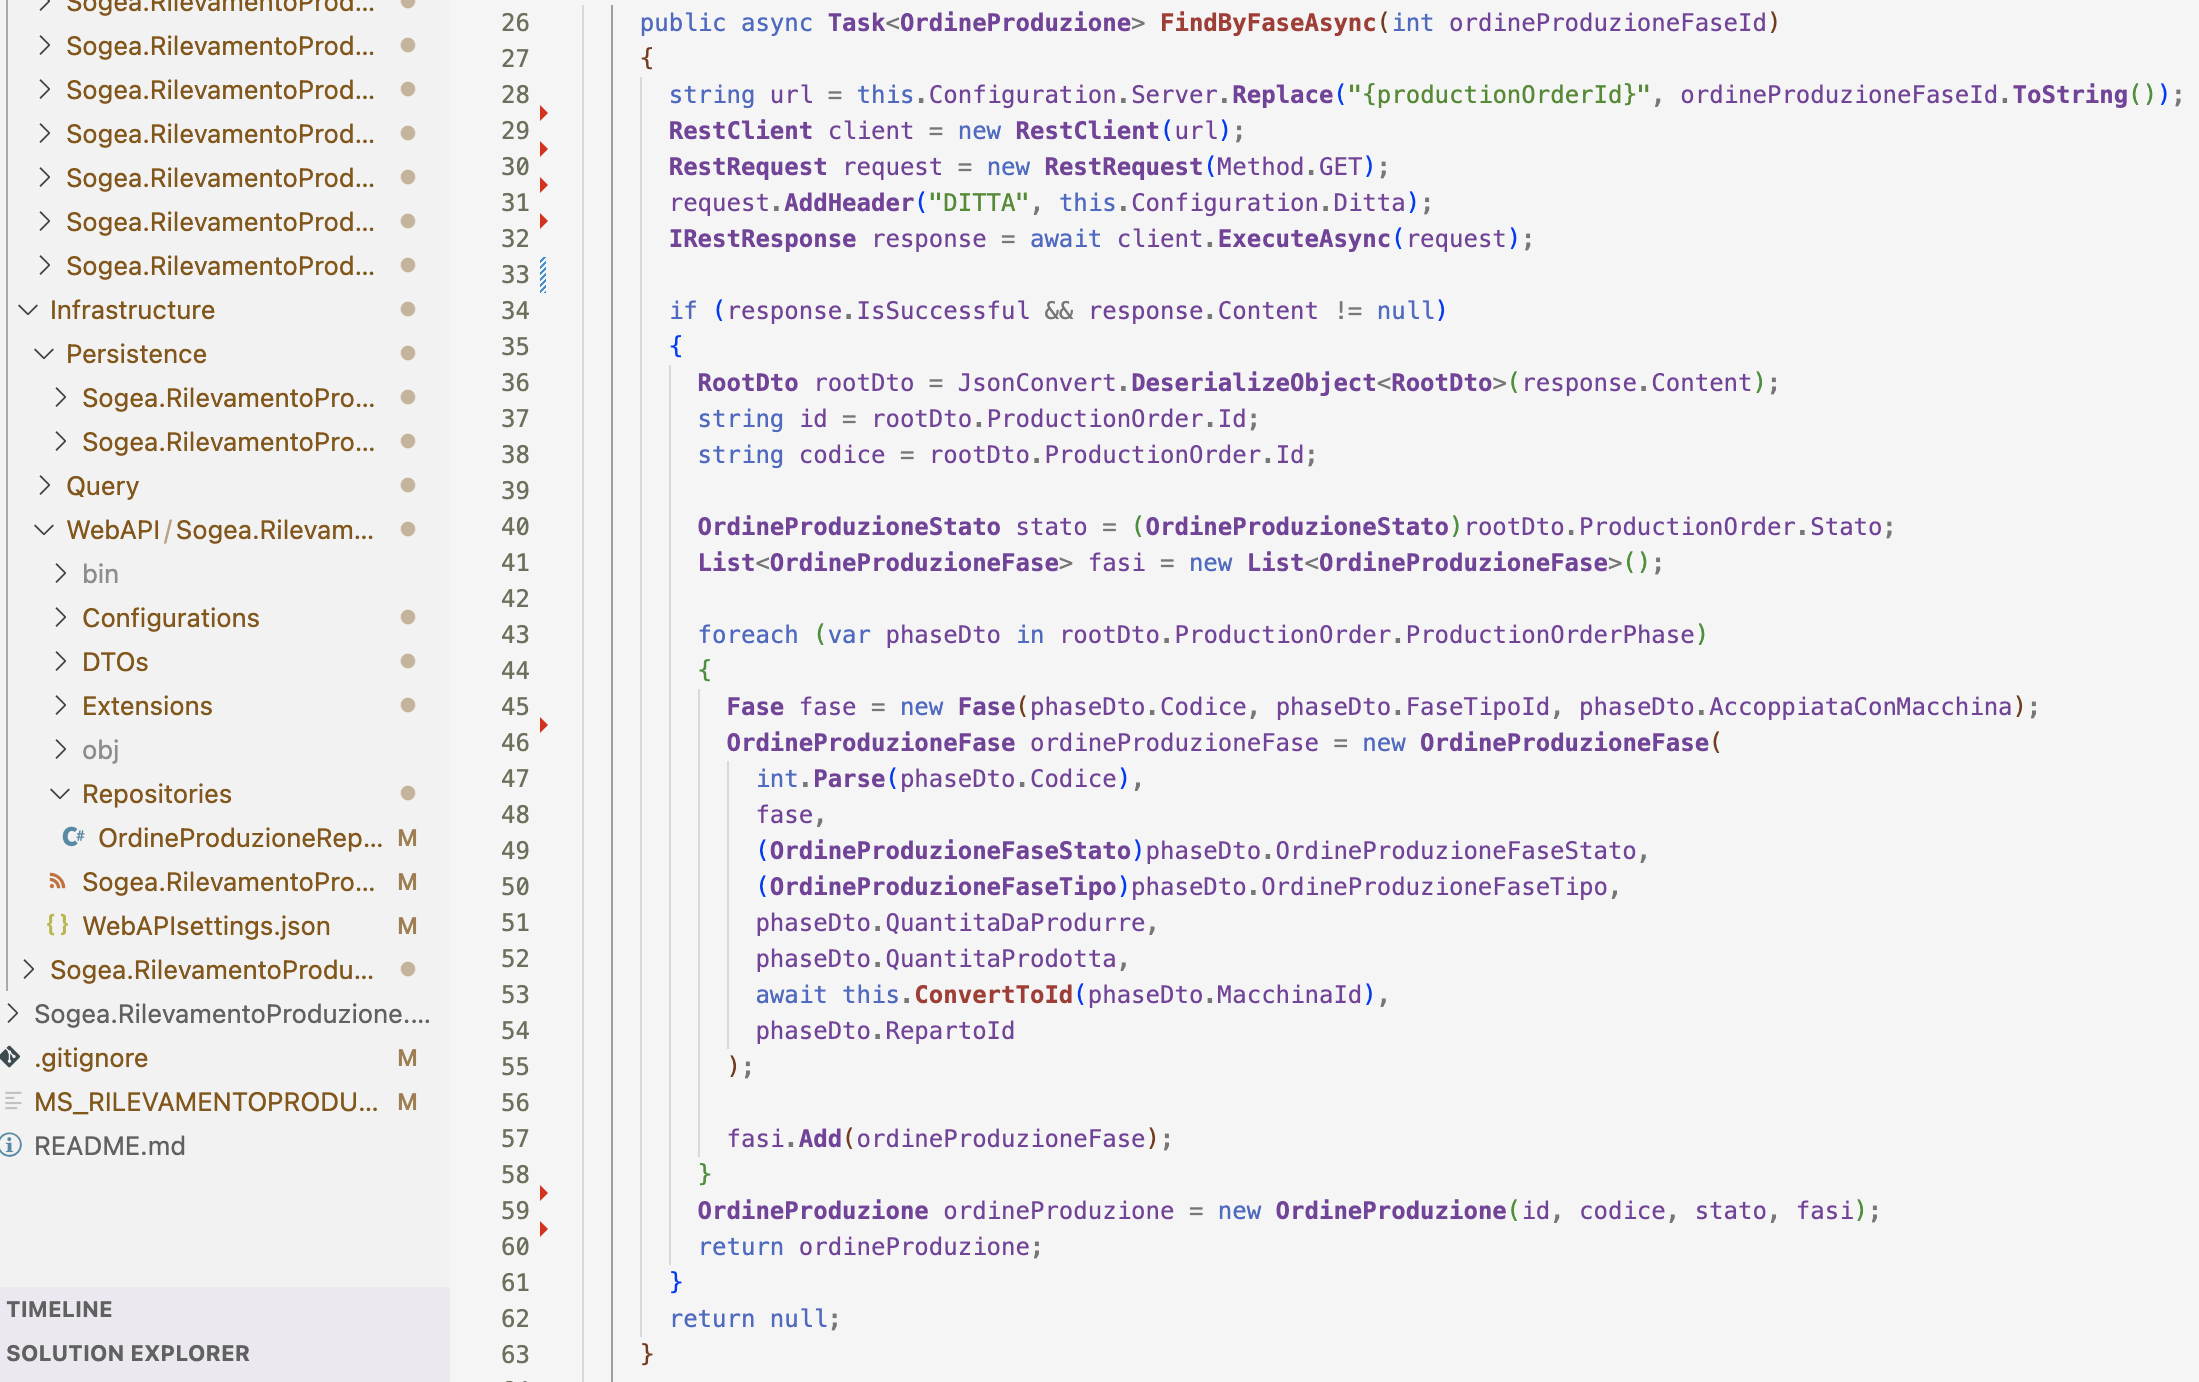
\includegraphics[width=1\linewidth]{BCS-Tessi//images/api.png}
            \caption{Implementazione dell'API per la comunicazione tra \texttt{OrdineProduzioneFase} e il \textit{database} monolitico}
            \label{fig:api}
        \end{figure}
        
        \vspace{0.2 em}
        \noindent Inizialmente, viene costruito dinamicamente l'\textbf{$endpoint_G$} della richiesta. L'$\textbf{URL}_G$ di destinazione viene generato sostituendo il segnaposto \texttt{productionOrderId} con l'identificativo effettivo della fase di produzione \texttt{(ordineProduzioneFaseId.ToString())}. Questa sostituzione avviene tramite il metodo \texttt{Replace} dell'oggetto \texttt{Configuration.Server}.

        \vspace{0.2 em}
        \noindent Viene dunque istanziato un \textit{client} REST (\texttt{new RestClient(url)}) e configurata una richiesta HTTP di tipo \textbf{GET} (\texttt{new RestRequest(Method.GET)}). La scelta del metodo GET è conforme alle convenzioni REST, dove GET rappresenta un'operazione di lettura che non modifica lo stato delle risorse sul \textit{server}.

        \vspace{0.2 em}
        \noindent Per contestualizzare la richiesta all'ambiente aziendale specifico, viene aggiunto un \textit{header} personalizzato denominato "\texttt{DITTA}" tramite il metodo \texttt{AddHeader}, utilizzando il valore memorizzato nella configurazione dell'applicazione.

        \vspace{0.2 em}
        \noindent L'esecuzione della richiesta avviene in modalità asincrona (\texttt{await client.ExecuteAsync} \\ \texttt{(request)}), una scelta che ottimizza l'utilizzo delle risorse di sistema evitando blocchi durante l'attesa della risposta dalla rete.

        \vspace{0.2 em}
        \noindent Durante l'elaborazione, il codice verifica il successo della risposta e la presenza di contenuti. In caso positivo, i dati \textbf{$JSON_G$} ricevuti vengono deserializzati in un oggetto \texttt{RootDto} tramite \texttt{JsonConvert.DeserializeObject<RootDto>}. Da questo DTO radice, vengono estratte le informazioni necessarie come identificativi, codici e stati dell'ordine di produzione. Questo è un perfetto esempio di come vengono strutturati gli aggregati nel contesto DDD. 

        \vspace{0.2 em}
        \noindent Nel DDD, gli aggregati rappresentano raggruppamenti di entità e oggetti di valore che vengono trattati come un'unità coesa per garantire l'integrità dei dati. Qui vediamo come i dati provenienti da un sistema esterno (in formato JSON) vengono prima trasformati in un DTO neutro (\texttt{RootDto}), che agisce come struttura intermedia, e poi progressivamente ricostruiti negli oggetti di dominio veri e propri (\texttt{OrdineProduzione}, \texttt{OrdineProduzioneFase}, \texttt{Fase}). Questa operazione è visibile nella Figura \ref{fig:rootdto}.

        \begin{figure}[H]
            \centering
            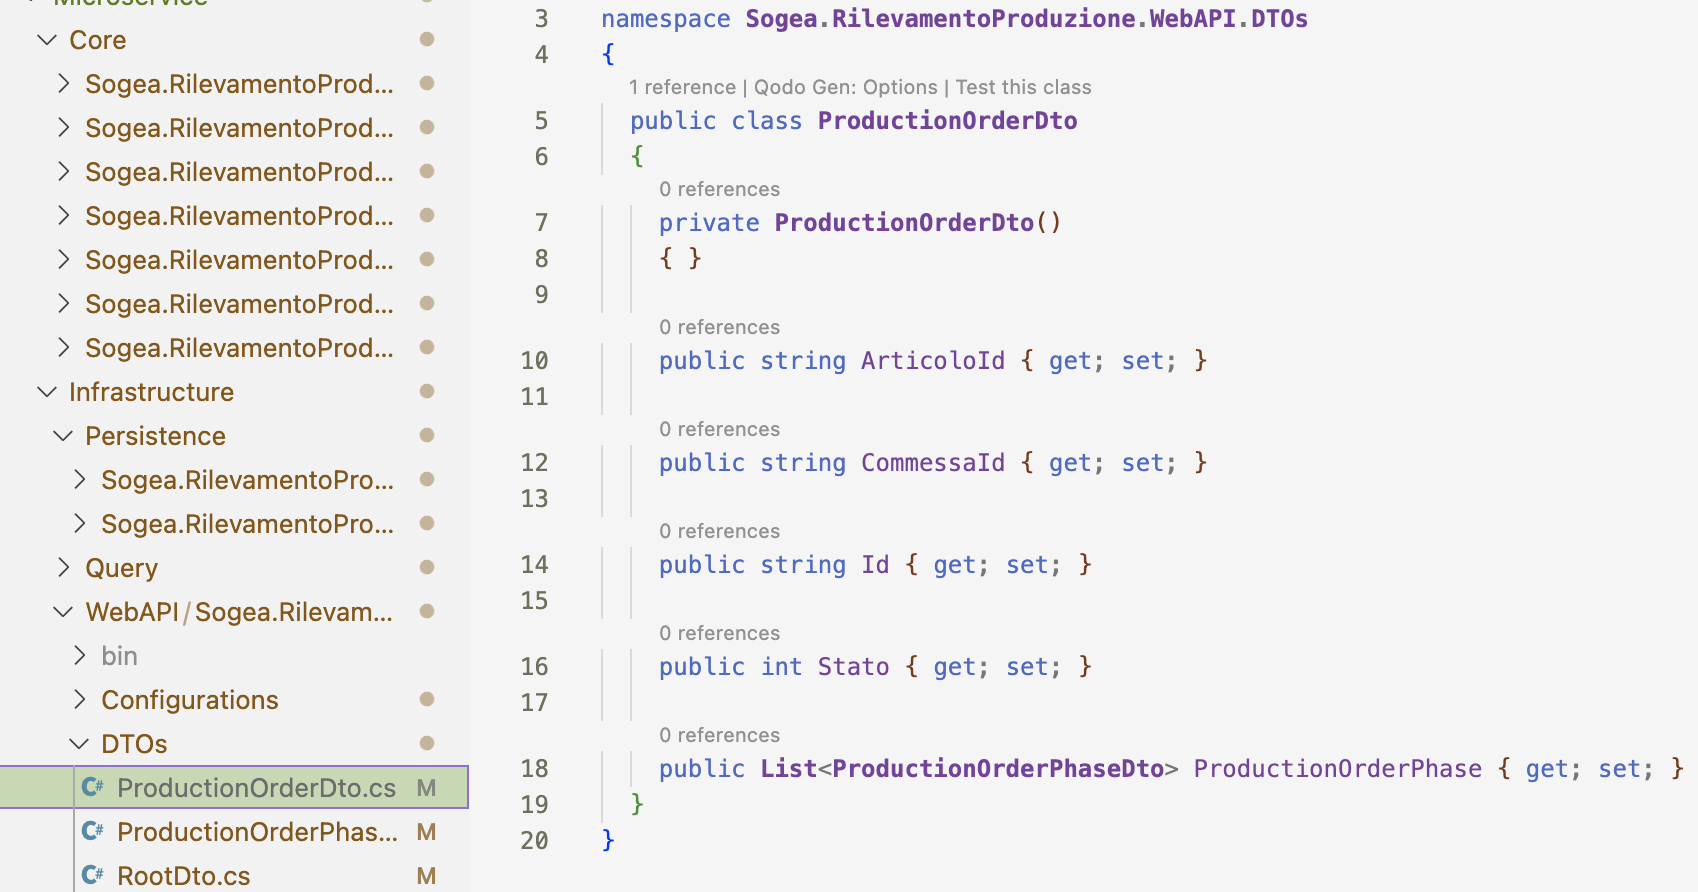
\includegraphics[width=1\linewidth]{BCS-Tessi//images/rootdto.png}
            \caption[Definizione della classe \texttt{ProductionOrderDto} e aggregati]{Definizione della classe \texttt{ProductionOrderDto} contenente le proprietà principali e le relazioni con le fasi degli ordini di produzione nel sistema, nonché la relazione in quanto aggregato. }
            \label{fig:rootdto}
        \end{figure}

        \vspace{0.2 em}
        \noindent Tornando alla Figura \ref{fig:api}, particolarmente interessante è la sezione di codice che itera attraverso le fasi dell'ordine di produzione (\texttt{foreach (var phaseDto in rootDto.ProductionOrder} \texttt{.ProductionOrderPhase)}). Per ciascuna fase, viene creato un nuovo oggetto \texttt{Fase} con i dettagli estratti dal DTO, seguito dalla creazione di un oggetto \texttt{OrdineProduzioneFase} completo di tutti i dati necessari.

        \vspace{0.2 em}
        \noindent Infine, tutti gli oggetti \texttt{OrdineProduzioneFase} vengono aggregati in una lista e utilizzati per costruire l'oggetto \texttt{OrdineProduzione} completo, che viene restituito come risultato dell'operazione. In caso di insuccesso della richiesta o in assenza di dati validi, il metodo restituisce \texttt{null}.

        \vspace{0.2 em}
        \noindent Questa implementazione dimostra un'efficace integrazione tra sistemi distribuiti, ottimizzando le comunicazioni e riducendo la duplicazione di richieste di dati attraverso un'interfaccia REST ben strutturata.

        \subsubsection{Change Data Capture}
        \vspace{0.2 em}
        \noindent Per affrontare invece la problematica della sincronizzazione dei dati, ho potuto esplorare e implementare un'architettura specializzata basata sulla tecnologia \textbf{Debezium}, una piattaforma di \textbf{\textit{Change Data Capture}} (\textbf{CDC}), approfondita nella Sezione 1.7. 

        \vspace{0.2 em}
        \noindent L'architettura di sincronizzazione adottata ha integrato Debezium con \textbf{RabbitMQ}, quest'ultimo utilizzato come \textit{message broker }per la gestione efficiente del flusso di informazioni. Questa combinazione tecnologica ha consentito la realizzazione di un sistema di code (inteso come liste) di messaggi altamente reattivo, in grado di catturare e propagare le modifiche ai dati nel momento stesso in cui queste venivano apportate nel sistema di origine.

        \vspace{0.2 em}
        \noindent Il principio operativo di questa soluzione si basa sul meccanismo di CDC, attraverso il quale Debezium monitora continuamente il \textit{log} delle transazioni del \textit{database}, identifica le operazioni di inserimento, aggiornamento o eliminazione dei dati e trasforma queste informazioni in eventi che vengono successivamente instradati attraverso RabbitMQ verso i sistemi destinatari, come si può osservare in Figura \ref{fig:queue}.

        \begin{figure}[H]
            \centering
            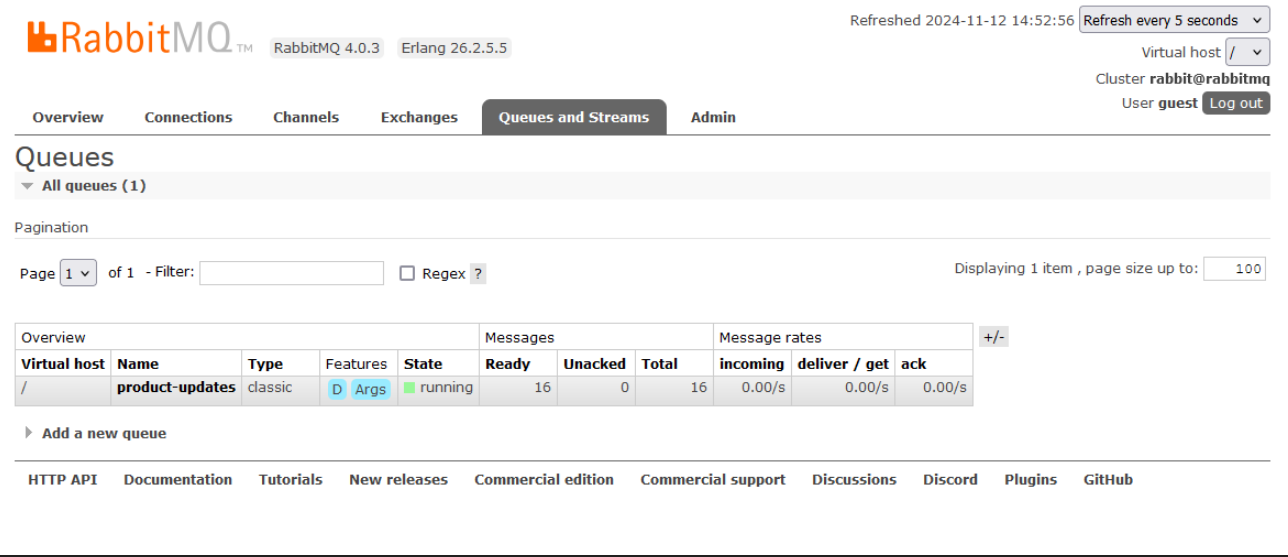
\includegraphics[width=1\linewidth]{BCS-Tessi//images/queue.PNG}
            \caption{Coda implementata con Debezium e gestita da RabbitMQ.}
            \label{fig:queue}
        \end{figure}

        \noindent L'implementazione dunque si è svolta senza particolari difficoltà, seguendo le attività di progettazione precedentemente definite. Rispetto alla previsione iniziale illustrata nella Figura \ref{fig:product-backlog}, avevo stimato di implementare circa il 73\% dei requisiti individuati. Tuttavia, al termine dello sviluppo, ho potuto constatare di aver raggiunto un 76\%, superando leggermente le aspettative iniziali.  

        \vspace{0.2 em}
        \noindent In particolare, l'esplorazione di \textbf{Debezium} era inizialmente prevista solo a livello teorico, ma sono riuscita anche a soddisfare i primi requisiti per la sua implementazione, ponendo le basi per l'adozione completa di questo \textit{framework} nell'applicazione del \textit{pattern} \textit{Change Data Capture} (CDC). 

        
        \subsection{Verifica e validazione}
        Il processo di verifica del \textit{software} è stato articolato in più fasi, iniziando dal controllo delle singole unità di codice per poi estendersi all’intero sistema, come illustrato nella Sezione 1.6.4.  

        \vspace{0.2 em}
        \noindent In SogeaSoft S.r.l., è prassi consolidata che qualsiasi modifica al codice venga sottoposta a revisione prima di essere integrata nel \textit{branch} stabile di sviluppo. Nello specifico, le modifiche devono essere pubblicate tramite una \textit{Pull Request} su Microsoft Azure e sottoposte alla verifica di un altro sviluppatore.

        \vspace{0.2 em}
        \noindent Quando viene aperta una \textit{Pull Request}, viene automaticamente avviata una \textit{pipeline} di \textit{test} sulla piattaforma Microsoft Azure. In questo ambiente, il codice viene compilato e sottoposto a \textit{test} automatici per verificarne la correttezza.  

        \vspace{0.2 em}
        \noindent Per tutti i \textit{task} rilevanti, ho provveduto a scrivere una serie di \textbf{\textit{test} unitari} volti a garantire il corretto funzionamento delle logiche definite durante le attività di progettazione. In SogeaSoft S.r.l. non sono previsti requisiti minimi di copertura per i \textit{test} unitari; tuttavia, ho scelto autonomamente di raggiungere il 100\% di copertura per tutte le funzionalità da me sviluppate. Questo approccio mi ha permesso di scrivere codice più solido e aderente alle specifiche progettuali.

        \vspace{0.2 em}
        \noindent Oltre ai \textit{test} unitari, ho eseguito anche \textbf{\textit{test} di integrazione}, concentrandomi in particolare sulla verifica del corretto funzionamento delle chiamate REST, su cui si basa gran parte del sistema. Questi \textit{test} avevano l'obiettivo di garantire che le funzionalità sviluppate fossero correttamente esposte nell'ambiente \textit{server} e rispondessero in modo adeguato alle richieste.  

        \vspace{0.2 em}
        \noindent Per la verifica e la documentazione delle API, ho utilizzato \textbf{Swagger}, descritto più nel dettaglio nella Sezione 1.7. Questo \textit{framework} mi ha permesso di monitorare in tempo reale il comportamento delle nuove implementazioni, fornendo un'interfaccia intuitiva per testare i servizi esposti. Il funzionamento di Swagger è illustrato nella Figura \ref{fig:swagger}.  

        \vspace{0.2 em}
        \noindent Per quanto riguarda i \textbf{\textit{test} di sistema}, le sessioni di \textit{Sprint Review} hanno rappresentato un'importante occasione di verifica, durante la quale le funzionalità sviluppate venivano sottoposte a un processo di valutazione strutturato. Questo momento coinvolgeva attivamente il \textit{Product Owner}, garantendo un confronto diretto sulla conformità delle implementazioni rispetto ai requisiti iniziali.  

        \vspace{0.2 em}
        \noindent Durante queste revisioni, oltre al \textit{Product Owner}, erano presenti tutti i membri del \textit{team} di sviluppo che interagivano con il microservizio in questione. Il \textit{Product Owner}, essendo in contatto diretto con gli \textit{stakeholder} e gli esperti di dominio, ha svolto il ruolo di intermediario, assicurando che le soluzioni implementate rispondessero alle esigenze aziendali.

        \vspace{0.2 em}
        \noindent L'azienda, avendo già un quadro chiaro delle richieste degli \textit{stakeholder}, è stata in grado di valutare con precisione il livello di soddisfacimento dei requisiti. Questo approccio ha permesso di ottenere un riscontro immediato e di identificare eventuali aree di miglioramento prima del rilascio definitivo, favorendo un ciclo di sviluppo iterativo e allineato alle necessità del \textit{business}.
        
        \begin{figure}[H]
            \centering
            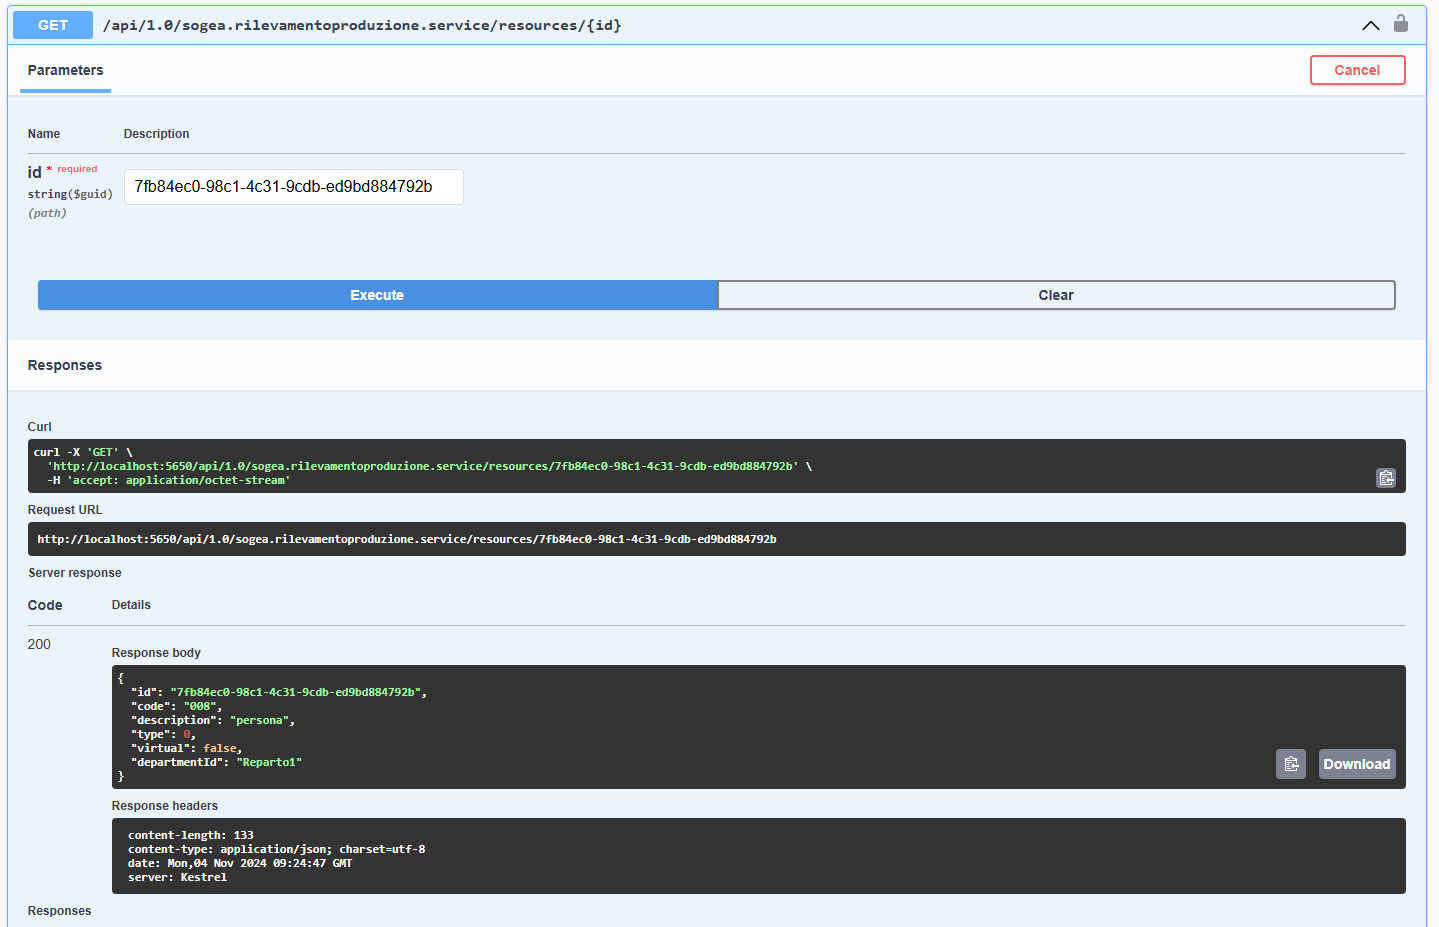
\includegraphics[width=1\linewidth]{BCS-Tessi//images/swagger.PNG}
            \caption{Schermata d'esempio di Swagger per la lettura di un dato.}
            \label{fig:swagger}
        \end{figure}

        \vspace{0.2 em}
        \noindent Come anticipato nella Sezione 1.6.4, il processo di validazione fornisce evidenza oggettiva sulle capacità del \textit{software} di soddisfare le aspettative e i bisogni del committente. 

        \vspace{0.2 em}
        \noindent Data la natura accademica del mio \textit{stage}, non sono state condotte validazioni formali che avrebbero previsto il coinvolgimento diretto degli \textit{stakeholder} esterni o di un \textit{domain expert}.  

        \vspace{0.2 em}
        \noindent Nel mio caso, la \textbf{validazione} del lavoro svolto è stata effettuata da diverse figure, a seconda della rilevanza degli avanzamenti apportati: il \textit{Product Owner}, il \textit{Team Leader} (che ha ricoperto anche il ruolo di mio \textit{tutor} aziendale) e, in alcuni casi, gli altri sviluppatori. Sebbene un’attività simile si sia già svolta durante i test di sistema, la validazione avrebbe richiesto un processo più strutturato e formale.  

        \vspace{0.2 em}
        \noindent L'obiettivo della validazione è verificare che il \textit{software}, in specifiche condizioni operative, sia in grado di soddisfare gli scopi per cui è stato progettato. Per questo motivo, è essenziale il coinvolgimento diretto degli \textit{stakeholder}. Di conseguenza, si può affermare che la vera validazione sarà effettuata in autonomia da SogeaSoft S.r.l., mentre il mio contributo si è limitato a un momento  preliminare di verifica interna.

        \vspace{0.2 em}
        \noindent Idealmente, la validazione di una funzionalità dovrebbe avvenire una sola volta, senza necessità di ripetere il processo. Per raggiungere questo obiettivo, il \textit{team} deve presentare prove oggettive, supportate dalla documentazione, che dimostrino la conformità della funzionalità agli scenari di esecuzione e il pieno soddisfacimento dei requisiti.  

        \vspace{0.2 em}
        \noindent Per garantire un processo futuro di validazione efficace, ho dedicato particolare attenzione alla manutenzione e all’aggiornamento della documentazione tecnica su Wiki Azure. In questo modo, il codice da me sviluppato è accompagnato da tutte le informazioni progettuali necessarie, facilitando la comprensione e la verifica delle soluzioni implementate.


    \section{Risultati raggiunti}
        \subsection{Il microservizio}
        L'estrazione del microservizio dal sistema monolitico preesistente ha raggiunto l'obiettivo prefissato, riuscendo preservare le funzionalità originarie pur trasferendole in un'architettura indipendente. L'esito positivo di questa migrazione è evidenziato dalla piena operatività del componente estratto, ora funzionante come entità autonoma al di fuori del contesto monolitico in cui era originariamente integrato. Al momento è possibile utilizzarlo solo tramite \textbf{Swagger}, ma l'azienda prevede di implementare anche i collegamenti con l'interfaccia più intuitiva attualmente in uso.

        \vspace{0.2 em}
        \noindent Il processo di estrazione ha richiesto l'implementazione di soluzioni tecniche che, sotto il profilo dell'eleganza architetturale, non sono perfette. Tuttavia, questi compromessi sono stati consapevolmente accettati in considerazione dell'obiettivo primario del progetto, che consisteva nell'estrazione funzionale del microservizio piuttosto che nella realizzazione di un'architettura ideale dal punto di vista teorico.

        \vspace{0.2 em}
        \noindent Al termine del periodo di \textit{stage}, il microservizio estratto ha raggiunto il livello di autonomia desiderato, pur mantenendo specifici canali di comunicazione con il sistema monolitico originario per garantire la continuità dei processi aziendali. Questa configurazione ha consentito al servizio di assumere la responsabilità esclusiva della gestione dei \texttt{rilevamenti} e delle \texttt{lavorazioni} associate alle \texttt{fasi} produttive, interfacciandosi con il sistema di gestione degli \texttt{ordini di produzione} e delle relative fasi (\texttt{OrdineProduzioneFase}), come è possibile osservare nella Figura \ref{fig:final-Swagger}.
        
        \begin{figure}
            \centering
            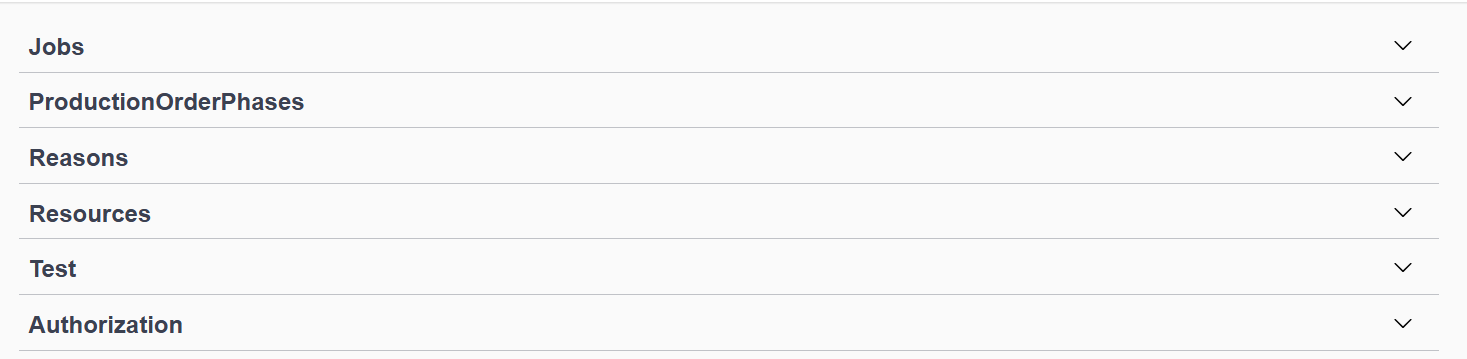
\includegraphics[width=1\linewidth]{BCS-Tessi//images/FinalSwagger.PNG}
            \caption{Schermata iniziale di Swagger per la gestione del microservizio \texttt{MS\_Rilevamento}}
            \label{fig:final-Swagger}
        \end{figure}

        \vspace{0.2 em}
        \noindent L'estrazione del microservizio ha prodotto un significativo miglioramento nell'efficienza operativa dell'organizzazione, risolvendo problematiche strutturali del sistema precedente, trattate nella Sezione 3.2.1. Inoltre, rispetto alle misurazioni su velocità ed efficienza citate nella Sezione 3.2.2, abbiamo osservato un miglioramento non indifferente soprattutto rispetto all'aggiornamento dei dati in tempo reale. 

        \vspace{0.2 em}
        \noindent Infatti, ella configurazione precedente di SAI, l'aggiornamento dei dati avveniva attraverso procedure \textit{batch} notturne, ossia di estrazione di un grande gruppo (\textit{batch}) di dati, eseguite ogni notte, imponendo un ritardo sistematico di 24 ore nella disponibilità delle informazioni aggiornate. Questa latenza costituiva un ostacolo significativo per gli operai, perché questa operazione era spesso soggetta a errori e un operaio doveva attendere diverse ore la risoluzione del problema. 

        \vspace{0.2 em}
        \noindent L'implementazione della tecnologia Debezium ha rivoluzionato questo paradigma, introducendo un meccanismo di aggiornamento in tempo reale che elimina questa latenza. Ciò ha permesso ai lavoratori di accedere immediatamente ai dati aggiornati, senza dover attendere l'esecuzione delle procedure \textit{batch}. Tuttavia, questo cambiamento ha comportato un aumento del costo computazionale. Rispetto alle previsioni iniziali sul \textit{Return on Investment}, il beneficio derivante dall’incremento della velocità e dalla riduzione della necessità di intervento umano per la risoluzione di problemi ha compensato i costi aggiuntivi, portando a un bilancio complessivo neutro, senza un guadagno significativo. 

        \vspace{0.2 em}
        \noindent Infatti questa transizione verso un modello \textit{event-$driven_G$}, ossia una rilevazione e gestione di eventi immediata, comporta un inevitabile compromesso in termini di consumo di risorse computazionali. La maggiore reattività del sistema si traduce in un più intenso utilizzo dell'infrastruttura, richiedendo un bilanciamento attento tra benefici operativi e costi infrastrutturali. Considerando questo \textit{trade-off}, l'implementazione della sincronizzazione in tempo reale è stata strategicamente limitata ai soli dati per i quali la tempestività dell'aggiornamento rappresenta un requisito critico per i processi aziendali. 

        
        \subsection{Risultati quantitativi}
        Durante il periodo di \textit{stage}, ho conseguito con successo \textbf{tre} dei quattro obiettivi obbligatori inizialmente concordati, unitamente all'obiettivo facoltativo. L'obiettivo classificato come desiderabile non è stato affrontato, in seguito a una rivalutazione delle priorità progettuali. Questo ha privilegiato lo sviluppo del \textit{Proof of Concept} (PoC), ossia l'obiettivo facoltativo 1 (FA1), rispetto alla documentazione esaustiva dell'ecosistema dei servizi preesistenti e delle loro interdipendenze (OB3).

        \vspace{0.2 em}
        \noindent Questo cambiamento delle priorità delle attività si è rivelata funzionale al rispetto del vincolo temporale delle 304 ore allocate per l'esperienza formativa. La gestione del tempo ha inoltre consentito l'estensione delle attività oltre il perimetro inizialmente definito, permettendo la realizzazione di un prototipo funzionale che rappresenta l'evoluzione naturale del \textit{Proof of Concept} sviluppato.

        \vspace{0.2 em}
        \noindent I risultati tangibili prodotti durante il periodo di \textit{stage} comprendono:
        \begin{itemize}
            \item un elaborato di analisi della letteratura riguardo le metodologie di migrazione verso architetture a microservizi;
            \item un documento tecnico sui \textit{pattern} di migrazione, con particolare enfasi sugli approcci ritenuti più pertinenti per il contesto specifico di SogeaSoft S.r.l.;
            \item un'analisi formale dei requisiti che sintetizza le esigenze funzionali e non funzionali identificate;
            \item 5826 linee di codice sorgente, sottoposte a processi di verifica e successivamente integrate nel \textit{branch} di sviluppo del progetto.
        \end{itemize}
        
    \section{Sviluppi futuri}
    Il progetto di \textit{stage} da me intrapreso riveste una particolare rilevanza per SogeaSoft S.r.l. in quanto si inserisce in un contesto di crescente esigenza di innovazione e miglioramento del sistema \textit{software} SAIonWeb. In seguito all'acquisizione da parte di Bluenext S.r.l., come descritto nella Sezione 1.1, l'applicativo è destinato a gestire un numero sempre maggiore di clienti. Questa evoluzione comporta la necessità di aggiornamenti più frequenti e tempestivi, nonché l'adattamento del \textit{software} alle specifiche esigenze aziendali e al relativo dominio di riferimento.  

    \vspace{0.2 em}
    \noindent Un aspetto cruciale risiede nella capacità di garantire ai clienti l'accesso ai dati in tempo reale, superando l'attuale limite che impone tempi di attesa di 24 ore per ottenere i dati del giorno precedente. Per raggiungere tale obiettivo, risulta imprescindibile scomporre il resto dell'architettura monolitica esistente e procedere verso una migrazione a un'architettura completamente basata su microservizi.  

    \vspace{0.2 em}
    \noindent Immagino che la prima cosa che caratterizzerà anche i progetti di \textit{stage} futuri sarà l'approfondimento della tecnologia Debezium, proprio a questo proposito. Ma non solo, anche l'esplorazione di nuovi \textit{pattern} risulta fondamentale. Dato che potenzialmente per ogni \textit{bounded context} può corrispondere un microservizio, come farli comunicare, come poterli estrarre, quali compromessi attuare sono sfide che SogeaSoft S.r.l. dovrà affrontare. 

     \vspace{0.2 em}
     \noindent In questo contesto dunque, il progetto di \textit{stage} ha costituito un primo passo significativo verso l'obiettivo più ampio della migrazione completa. Pur rappresentando solo una parte del progetto di lungo termine, il lavoro svolto ha permesso di delineare e testare approcci metodologici e tecnici che potranno essere riutilizzati e ampliati nelle fasi successive. La mia attività ha quindi contribuito a gettare le basi per un percorso di trasformazione che, nel medio-lungo periodo, porterà a una maggiore flessibilità e scalabilità del sistema SAIonWeb.
    
    
    